%%%%%%%%%%%%%%%%%%%%%%%%%%%%%%%%%%%%%%%%%
% Short Sectioned Assignment LaTeX Template Version 1.0 (5/5/12)
% This template has been downloaded from: http://www.LaTeXTemplates.com
% Original author:  Frits Wenneker (http://www.howtotex.com)
% License: CC BY-NC-SA 3.0 (http://creativecommons.org/licenses/by-nc-sa/3.0/)
%%%%%%%%%%%%%%%%%%%%%%%%%%%%%%%%%%%%%%%%%

%----------------------------------------------------------------------------------------
%	PACKAGES AND OTHER DOCUMENT CONFIGURATIONS
%----------------------------------------------------------------------------------------

\documentclass[paper=a4, fontsize=11pt]{scrartcl} % A4 paper and 11pt font size
% ---- Entrada y salida de texto -----

\usepackage[T1]{fontenc} % Use 8-bit encoding that has 256 glyphs
\usepackage[utf8]{inputenc}
%\usepackage[default]{sourcesanspro}
\usepackage{fourier} % Use the Adobe Utopia font for the document - comment this line to return to the LaTeX default
% ---- Idioma --------

\usepackage[spanish, es-tabla]{babel} % Selecciona el español para palabras introducidas automáticamente, p.ej. "septiembre" en la fecha y especifica que se use la palabra Tabla en vez de Cuadro

% ---- Code insertion ----
\usepackage{minted}
\usepackage[breakable]{tcolorbox} %Genera boxes, lo usamos para el codigo
\BeforeBeginEnvironment{minted}{\begin{tcolorbox}[breakable]}%
	\AfterEndEnvironment{minted}{\end{tcolorbox}}%
\BeforeBeginEnvironment{inputminted}{\begin{tcolorbox}[breakable]}%
	\AfterEndEnvironment{inputminted}{\end{tcolorbox}}%

\usepackage{xpatch} %permite abrir environments al ejecutar ciertos comandos

\xpretocmd{\inputminted}{\begin{tcolorbox}}{}{}%
	\xapptocmd{\inputminted}{\end{tcolorbox}}{}{}%

\setminted{
fontsize=\small,
breaklines,
breaksymbolleft=
}
% ---- Otros paquetes ----
\usepackage{dirtree}
\usepackage{vmargin}

\usepackage{url} % ,href} %para incluir URLs e hipervínculos dentro del texto (aunque hay que instalar href)
\usepackage{hyperref} % ,href} %para incluir URLs e hipervínculos dentro del texto (aunque hay que instalar href)
\hypersetup{
	colorlinks=true,
	linkcolor=blue,
	filecolor=magenta,      
	urlcolor=blue,
}

\usepackage{xcolor}
\definecolor{light-gray}{gray}{0.95}
\definecolor{alizarin}{rgb}{0.82, 0.1, 0.26}
\definecolor{nyellow}{rgb}{0.91, 0.656, 0.0}
%\definecolor{indigo}{rgb}{0.29, 0.0, 0.51}
%	\textcolor{red}{p}
%	\textcolor{orange}{r}
%	\textcolor{yellow}{a}
%	\textcolor{green}{c}
%	\textcolor{blue}{t}
%	\textcolor{indigo}{i}
%	\textcolor{violet}{c}
%	\textcolor{red}{a}
%	\textcolor{orange}{s}
%	\textcolor{yellow}{,}
%	\textcolor{green}{I}
%	\textcolor{blue}{S}
%	\textcolor{indigo}{E}

\usepackage{amsmath,amsfonts,amsthm} % Math packages
%\usepackage{graphics,graphicx, floatrow} %para incluir imágenes y notas en las imágenes
\usepackage{graphics,graphicx, float} %para incluir imágenes y colocarlas
\usepackage[export]{adjustbox}
\graphicspath{{imagenes/}}

% Para hacer tablas comlejas
%\usepackage{multirow}
%\usepackage{threeparttable}

%\usepackage{sectsty} % Allows customizing section commands
%\allsectionsfont{\centering \normalfont\scshape} % Make all sections centered, the default font and small caps

%Remove warnings
\usepackage{silence}
\WarningFilter{scrartcl}{Usage of package `fancyhdr'}

\usepackage{fancyhdr} % Custom headers and footers
\pagestyle{fancyplain} % Makes all pages in the document conform to the custom headers and footers
\fancyhead{} % No page header - if you want one, create it in the same way as the footers below
\fancyfoot[L]{} % Empty left footer
\fancyfoot[C]{} % Empty center footer
\fancyfoot[R]{\thepage} % Page numbering for right footer
\renewcommand{\headrulewidth}{0pt} % Remove header underlines
\renewcommand{\footrulewidth}{0pt} % Remove footer underlines
\setlength{\headheight}{13.6pt} % Customize the height of the header

\numberwithin{equation}{section} % Number equations within sections (i.e. 1.1, 1.2, 2.1, 2.2 instead of 1, 2, 3, 4)
\numberwithin{figure}{section} % Number figures within sections (i.e. 1.1, 1.2, 2.1, 2.2 instead of 1, 2, 3, 4)
\numberwithin{table}{section} % Number tables within sections (i.e. 1.1, 1.2, 2.1, 2.2 instead of 1, 2, 3, 4)

\setlength\parindent{0pt} % Removes all indentation from paragraphs - comment this line for an assignment with lots of text

\newcommand{\horrule}[1]{\rule{\linewidth}{#1}} % Create horizontal rule command with 1 argument of height

\setmarginsrb{2 cm}{1 cm}{2 cm}{2 cm}{1 cm}{1.5 cm}{1 cm}{1.5 cm} %Aumenta los márgenes

%----------------------------------------------------------------------------------------
%	TÍTULO Y DATOS DEL ALUMNO
%----------------------------------------------------------------------------------------

\title{
	Práctica 3.b \\\vspace{1cm}
	Técnicas de Búsqueda basadas en Trayectorias para el
	Problema del Aprendizaje de Pesos en Características
 \vspace{1cm} \\
	El problema del Aprendizaje de Pesos en Características (APC)	\vspace{1cm} \\
	Algoritmos BMB, ILS, VNS, ES e ILS-ES
	\hspace{1cm} 
 }   

\author{Yeray López Ramírez	}                             

\renewcommand*\contentsname{hola}

\makeatletter
\let\thetitle\@title
\let\theauthor\@author
\let\thedate\@date
\makeatother

%----------------------------------------------------------------------------------------
% DOCUMENTO
%----------------------------------------------------------------------------------------

\begin{document}
\begin{titlepage}
	\centering
	%\textsc{\LARGE Universidad de Granada}\\[2.0 cm]    
	
\includegraphics[scale = 0.6]{ugr.png}\\[1.0 cm]
	\rule{\linewidth}{0.2 mm} \\[0.4 cm]
	{ \huge \bfseries \thetitle}\\
	\rule{\linewidth}{0.2 mm} \\[1.5 cm]
	
	\begin{minipage}{0.5\textwidth}
		\begin{flushleft} \large
			\theauthor 
			123456789-Z \\
			\href{mailto:fulanito@correo.ugr.es}{fulanito@correo.ugr.es}
		\end{flushleft}
	\end{minipage}~
	\begin{minipage}{0.5\textwidth}
		\begin{flushright} \large
			Curso: 2022-23 \\
			Grupo A, 15:30 - 17:30 (Martes)                   
		\end{flushright}
	\end{minipage}\\[1 cm]
	
	{\small \thedate}\\[1 cm]
	
	\vfill
	
\end{titlepage}


\newpage %inserta un salto de página
\newcommand{\code}[1]{\colorbox{light-gray}{\textcolor{alizarin}{\texttt{#1}}}}
\newcommand{\high}[1]{\colorbox{light-gray}{\textcolor{nyellow}{\texttt{#1}}}}

\tableofcontents % para generar el índice de contenidos

\listoffigures

\listoftables

\newpage

%----------------------------------------------------------------------------------------
%	Cuestión 1
%----------------------------------------------------------------------------------------

\section{Descripción del problema}
El problema del Aprendizaje de Pesos en Características (APC) consiste en encontrar una combinación ponderada de un conjunto de características que maximice la precisión de un clasificador y minimice su complejidad. En este problema, se busca determinar la importancia relativa de cada característica para mejorar la eficiencia computacional y la precisión del modelo. El objetivo es encontrar un vector de pesos que asigne valores más altos a las características más importantes y valores más bajos a las características menos relevantes, y que permita eliminar aquellas características que no aporten información relevante para la tarea de clasificación. \\

En otras palabras, el APC busca determinar qué características son más relevantes para un problema dado y cómo combinarlas de manera óptima para obtener el mejor rendimiento de un modelo. \\

El modelo clasificador utilizado en este problema es el 1-NN, el cual es un método de aprendizaje supervisado que clasifica una instancia basándose en la clase de su vecino más cercano en el conjunto de entrenamiento. Además, se utilizará la técnica de validación leave-one-out para evaluar el desempeño del clasificador. La función objetivo que se busca maximizar será una combinación de medidas de precisión (tasa\_clas) y complejidad del clasificador (tasa\_red), dando como resultado el fitness.\\

Los conjuntos de datos utilizados en este problema son \textbf{diabetes}, \textbf{ozone-320} y \textbf{spectf-heart}. Diabetes es un conjunto de datos médicos que contiene información sobre pacientes con diabetes, como su edad, índice de masa corporal, presión arterial y resultados de pruebas de laboratorio, entre otros. Ozone-320 es un conjunto de datos de calidad del aire que contiene mediciones de ozono y otros contaminantes atmosféricos en diferentes ciudades de Estados Unidos. Spectf-heart es un conjunto de datos médicos que contiene información sobre pacientes que se sometieron a pruebas de diagnóstico por imágenes para enfermedades cardíacas. Todos los datasets tienen 2 etiquetas: negativo/positivo o 1.0/2.0 para indicar la clase del vector de características.  
\newpage

\section{Descripción de la aplicación de los algoritmos}
Los algoritmos utilizados para resolver el problema del Aprendizaje de Pesos en Características (APC) son Metaheurísticas que buscan optimizar una función objetivo que combina la precisión y la complejidad del clasificador 1-NN diseñado utilizando un vector de pesos. En este problema, se busca encontrar el mejor subconjunto de características que permita obtener una alta tasa de clasificación y, al mismo tiempo, reducir la complejidad del modelo. \\

Para aplicar estos algoritmos al problema de APC, se utilizó el esquema de representación basado en un vector de tamaño n con valores en [0, 1] que indican el peso asociado a cada característica. La función objetivo fue definida como la combinación con pesos de la tasa de acierto y la tasa de reducción de características del clasificador 1-NN diseñado empleando el vector de pesos. El objetivo es maximizar esta función, multiplicando la tasa de acierto por 0.8 y la tasa de reducción por 0.2, para dar mayor importancia a la clasificación que a la reducción de características.
\[\text{Fit} = 0.8 \cdot \text{precision} + 0.2 \cdot \text{reduction}\]

La implementación en pseudocódigo de la \textbf{función objetivo}:

\begin{minted}{text}
Input(Conjunto de Entrenamiento "Train", Conjunto de Prueba "Test", Vector de pesos W)
Inicio
    aciertos <- CLASIFICAR(Train, Test, W)
    tasa_clas <- aciertos/tamaño_test
    tasa_red <- PESOS_MENOR_UMBRAL(W, 0.1)
    DEVOLVER(0.8·tasa_clas + 0.2·tasa_red)
Fin
\end{minted}

Donde CLASIFICAR llama al modelo clasificador de vecinos 1-NN. El clasificador 1-NN (del inglés "Nearest Neighbor") es un algoritmo de clasificación que se basa en encontrar el vecino más cercano a un ejemplo de prueba en un conjunto de datos de entrenamiento, y asignarle la etiqueta del vecino como la etiqueta del ejemplo de prueba. En otras palabras, el algoritmo encuentra el ejemplo de entrenamiento más cercano al ejemplo de prueba en términos de \textbf{distancia}, y le asigna la etiqueta del ejemplo de entrenamiento como la etiqueta del ejemplo de prueba. La implementación en pseudocódigo del \textbf{clasificador 1NN} es:

\begin{minted}{c++}
Input(Vector características "A", Conjunto Entrenamiento "T", pesos W)
Inicio
    Inicializar min_distancia(INFINITY) y min_index(-1)
    Para cada vector B en T
        distancia <- DISTANCIA_EUCLIDEA(A,B,W)
        Si distancia es menor que min_distancia
            entonces min_index <- T.indice y min_distancia <- distancia
     DEVOLVER(T.GET_ETIQUETA(min_index))
Fin
\end{minted}

Cuando la función objetivo llama a CLASIFICAR lo que realmente hace es ejecutar el clasificador 1-NN con todo el conjunto de prueba. \\

Tanto el clasificador como el algoritmo de Greedy y la Búsqueda Local requieren del cálculo de la distancia entre los ejemplos. La \textbf{distancia euclidiana} es una medida de distancia comúnmente utilizada en problemas de clasificación y agrupamiento. Esta distancia mide la distancia geométrica entre dos puntos en un espacio n-dimensional. Se calcula como la raíz cuadrada de la suma de las diferencias al cuadrado de cada coordenada:

\[d(p,q) = \sqrt{(e^1_1 - e^1_2)^2 + (e^2_1 - e^2_2)^2 + ... + (e^n_1 - e^n_2)^2} =  \sqrt{\sum_{i=1}^n (e^i_1 - e^i_2)^2}\]

En el contexto del clasificador 1-NN, la distancia euclidiana se utiliza para medir la similitud entre dos ejemplos, uno del conjunto de entrenamiento y otro del conjunto de prueba. La idea es comparar el ejemplo de prueba con cada uno de los ejemplos de entrenamiento, y seleccionar la etiqueta del ejemplo más cercano al de prueba.\\

Los pesos w se usan para ajustar la importancia de cada atributo en el cálculo de la distancia euclidiana. Si un atributo tiene un peso alto, entonces su valor tendrá un mayor impacto en la medida de distancia. Por lo tanto, es importante elegir los pesos adecuados para obtener una buena precisión de clasificación. En algunos casos, ciertos atributos pueden ser irrelevantes o redundantes, y su peso puede establecerse en cero para ignorarlos en el cálculo de la distancia. La implementación en pseudocódigo de la \textbf{distancia euclidiana ponderada}:

\begin{minted}{c++}
Input(Vector características "A", Vector características "B", Vector de pesos "W", Umbral=0.1)
Inicio
    Inicializa distancia(0)
    Para cada i en número de características
        Si el peso wi es menor al umbral
            salta la iteración
        Sino
            entonces dist <- wi + (Ai - Bi)²
      DEVUELVE(RAIZ_CUADRADA(dist))
Fin
\end{minted}

Y por último pero no menos el importante, la función de \textbf{leave one out}. El Leave One Out es un procedimiento para evaluar la capacidad predictiva de un modelo de clasificación utilizando todo el conjunto de datos para el entrenamiento y la validación. El proceso consiste en evaluar el modelo n veces, dejando un ejemplo fuera (leave one out) del conjunto de datos en cada iteración para su uso en la validación. El modelo se entrena con los n-1 ejemplos restantes y se utiliza para predecir el ejemplo que se dejó fuera. La precisión del modelo se mide mediante el número de predicciones correctas sobre el total de ejemplos que se dejaron fuera. La implementación en pseudocódigo del \textbf{LOO}:

\begin{minted}{c++}
Input(Conjunto de datos "C", Indice "i")
Inicio
    Dataset Loo <- C
    ELIMINAR_EJEMPLO(Loo, i)
    DEVOLVER(Loo)
Fin
\end{minted}


\section{Estructuras de datos y algoritmos}
\subsection{Estructura de Datos en C++}
En primer lugar, mencionar que se ha elegido el lenguaje de programación C++. Se han definido principalmente dos Estructuras que forman la base del programa:
\begin{itemize}
	\item Struct Ejemplo: contiene un vector de características y un string de etiqueta. Representa a cada individuo en los conjuntos de datos.
	\item Class Dataset: contiene un vector de Ejemplos y vector de etiquetas. Representa a todo el conjunto de datos, puede ser train o test según la lectura de los datos.
	
	\item Class Poblacion: contiene una matriz de poblacion donde cada fila representa un individuo de la misma, un vector de fitness donde guarda el valor de fitness de cada individuo y varios enteros con las posiciones al peor, segundo peor y mejor fitness.
\end{itemize}

En la lectura se aplicó el método de validación cruzada (cross-folding) para evaluar el rendimiento de los algoritmos de selección de características en el problema de Aprendizaje de Pesos en Características (APC). \\

Este método consiste en dividir el conjunto de datos en $k$ particiones de igual tamaño, donde una de las particiones se utiliza como conjunto de prueba y las $k-1$ particiones restantes se utilizan como conjunto de entrenamiento. Este proceso se repite $k$ veces, de tal manera que cada partición se utiliza exactamente una vez como conjunto de prueba. De esta forma, se obtiene una medida más robusta del rendimiento del algoritmo, ya que se evalúa el rendimiento sobre datos que no han sido utilizados para entrenar el modelo. \\

En nuestro problema se utilizó la validación cruzada con $k=5$, lo que significa que se dividieron los datos en 5 particiones de igual tamaño y se realizaron 5 iteraciones del proceso de entrenamiento y evaluación. Para cada iteración, se utilizó una partición diferente como conjunto de prueba y las demás particiones como conjunto de entrenamiento. Se promedió el rendimiento obtenido en las 5 iteraciones para obtener una medida general del rendimiento de cada algoritmo. \\

Para ayudar a la reproducibilidad y verificación de los algoritmos, se nos ha proporcionado los ficheros de datos ya divididos así que el método de lectura se limita a leerlos y aplicar la validación cruzada. La implementación en pseudocódigo del \textbf{método de lectura}:

\begin{minted}{c++}
Input(Una cadena "nombre", Conjunto de Datos "Train", Conjunto de Datos "Test", Indice de test "k")
Inicio
    Si nombre no es igual a "diabetes", "ozone-320" o "spectf-heart"
        entonces DEVOLVER(error)
    Sino
        inicializa train, test
        Para cada i hasta k
            f <- nombre + i
            Si i == k
                 entonces READ(test, f)
            en otro caso
                 READ(train, f)
     DEVOLVER(sucess)
Fin
\end{minted}

La función READ de cada conjunto de datos se encarga de leer el fichero $f$ e integrarlo en la estructura. Se ignoran todos los comentarios y se leen los datos como una matriz de Ejemplos.\\

\subsection{Algoritmos de Trayectoria}
Un algoritmo basado en trayectorias, también conocido como algoritmo de búsqueda de trayectorias, es un enfoque de resolución de problemas que se centra en encontrar una trayectoria o camino óptimo en un espacio de búsqueda.\\

Este tipo de algoritmo se utiliza principalmente en problemas de optimización, donde se busca encontrar la mejor solución dentro de un conjunto de posibles soluciones. La idea es explorar el espacio de búsqueda de manera iterativa, moviéndose de un estado a otro, evaluando la calidad de cada estado y eligiendo la mejor opción en función de un criterio objetivo.\\

La exploración de la trayectoria se realiza a través de movimientos sucesivos entre estados adyacentes en el espacio de búsqueda. Estos movimientos pueden ser determinados por una heurística específica o una mutación aleatoria de la población que guíe la búsqueda hacia soluciones prometedoras y no atascarse en óptimos locales.\\

Los algoritmos de trayectoria se diferencian de otros enfoques de optimización en que no exploran exhaustivamente todo el espacio de búsqueda, sino que se centran en una trayectoria particular que conduce a una solución óptima. Esto permite reducir el tiempo de búsqueda y encontrar soluciones aceptables en problemas complejos con grandes espacios de búsqueda.\\

Algunos ejemplos de algoritmos basados en trayectorias incluyen la búsqueda local (Búsqueda Local Reiterada, ILS), la búsqueda multiarranque básico (BMB), Búsqueda de vecindad variable (VNS),  el enfriamiento simulado (ES) y su versión iterativa (ILS-ES). Estos algoritmos tienen diferentes estrategias de búsqueda y características específicas que los hacen adecuados para diferentes tipos de problemas y requisitos de optimización.

\subsubsection{Búsqueda Local}
En el algoritmo de \textbf{búsqueda local} la solución inicial se generó de forma aleatoria utilizando una distribución uniforme en [0, 1], y el movimiento de cambio por mutación normal Mov(W,s) se utilizó como esquema de generación de vecinos en la Búsqueda Local. En cada iteración de la Búsqueda Local, se mutó una componente i del vector de pesos en un orden aleatorio distinto para cada solución, hasta que se alcanzó una solución mejor o se modificaron todas las posiciones una vez sin conseguir una mejora. Se implementa de la siguiente forma:
\begin{minted}{text}
Input(Conjunto de datos "Train")
Inicio
GENERAR_SOLUCION_INICIAL(Wact, Train.NUMERO_CARACTERÍSTICAS)
objetivoActual <- FUN_OBJETIVO(Train, Wact)
Inicializar iteraciones, iter_vecinos = 0, W = Wact
Mientras que iter_vecinos < 20*Sact.SIZE y iteraciones menor que 15,000
Vec_indices <- GENERAR_VECINDARIO(W.SIZE)
Inicializar bool mejora <- false
Para cada i en Vec_indices y mientras no haya mejora
GENERAR_VECINO(W, i, 0.8)
objetivo <- FUN_OBJETIVO(Train, W)
Si el objetivo es mayor que el actual
Inicializar iter_vecinos = 0
objetivoActual <- objetivo
Wact = W
mejora = true
iter_vecinos+1
iter+1

DEVOLVER(Wact)
\end{minted}
A continuación se describe con detalle los esquemas:
\begin{itemize}
	\item Generación de la solución inicial: usamos la librería \code{random.hpp} proporcionada, concretamente Random::get<std::vector>(0.0, 1.0, numCaracteristicas) que genera un vector aleatorio de números reales entre 0 y 1 de tamaño numCaracterísticas.
	\item Generación de vecindario: usamos la librería \code{random.hpp} para hacer un shuffle a los índices de pesos.
	\item Generación de vecinos: esta vez hay que tener más cuidado pues hay que sumar un vector Z con distribución normal y respetar la representación de los pesos [0,1]. Una implementación sencilla en pseudocódigo es la siguiente:
	\begin{minted}{c++}
Input(Pesos "W", indice "i", valor de "media" = 0, valor de" varianza" = 0.8)
Inicio
z <- DISTRIBUCION_NORMAL(0, SQRT(varianza))
Si Wi + z es mayor a 1
TRUNCAR(Wi, 1)
Si Wi + z es menor a 0
TRUNCAR(Wi, 0)
Si no
Wi <- Wi + z
DEVOLVER(W)
	\end{minted}
	
	\item Criterio de aceptación: se cumple cuando el objetivo del vecino generado es mayor que el actual, lo controlamos con el valor de mejora.
\end{itemize}

\newpage

\subsection{Algoritmo de Enfriamiento Simulado}
El algoritmo de enfriamiento simulado (Simulated Annealing) es una técnica de búsqueda por trayectoria utilizada para encontrar soluciones aproximadas a problemas de optimización combinatoria. Está inspirado en el proceso de enfriamiento de los materiales en metalurgia.\\

El algoritmo se basa en la idea de explorar el espacio de búsqueda permitiendo movimientos a soluciones vecinas, incluso si estas soluciones empeoran la función objetivo. Este enfoque permite evitar quedarse atrapado en óptimos locales y explorar regiones del espacio de búsqueda que podrían contener soluciones mejores.\\

Inicialmente, se utiliza una alta temperatura que permite aceptar soluciones empeorantes con una cierta probabilidad. A medida que avanza el algoritmo, la temperatura se reduce gradualmente, lo que disminuye la probabilidad de aceptar soluciones empeorantes y hace que el algoritmo converja hacia una solución óptima o cercana a ella.\\

Para aplicar el algoritmo debemos calcular varias componentes:

\begin{itemize}
 \item Temperatura inicial: debemos calcular la $t_0$ usando la siguiente fórmula:
 \begin{figure}[H]
 	\[
 	T_{0}= \frac{\mu \cdot C(S_0)}{-ln(\varphi)} 
 	\]
 	\caption{Fijar temperatura}
 \end{figure}
 donde:
 \begin{itemize}
 	\item $\mu$: es un valor 0.3 calculado experimentalmente.
 	\item $C(S_0)$ es el fitness de la solución inicial.
 	\item $\phi$ es un valor 0.2 que determina la probabilidad de obtener una solución peor.
 \end{itemize}
 
 Debemos asegurarnos de que no sea inferior a la temperatura final ($t_f=10^{-4}$) por ello si se diera el caso de que $t_0 < t_f$ lo que se haría es reducir más la temperatura final hasta cumplir la condición. En el pseudocódigo se llama \code{FijarTemperaturaZero(fitness)} que es tal cual la fórmula previa + condición para $t_f > t_0$.
 
 \item Calcular la beta: en el mecanismo de enfriamiento se requiere calcular la tasa de enfriamiento $\beta$ tal que:
 \begin{figure}[H]
 	\[
 	\beta = \frac{T_0 - T_f}{M \cdot T_0 \cdot T_f}
 	\]
 	\caption{Calcular beta}
 \end{figure}
 donde:
 \begin{itemize}
 	\item M: es el número de evaluaciones totales entre el número de vecinos $\frac{MAX\_EVAL}{MAX\_VECINOS}$.
 	\item $T_0$: es la temperatura inicial previamente calculada.
 	\item $T_f$: es la temperatura final, por defecto $10^{-4}$
 \end{itemize}
 En el pseudocódigo se llama a \code{CalculoBeta} que aplica la fórmula previa.
 
 \item Calcular el mecanismo de enfriamiento: es el método que simula el enfriamiento de la temperatura. La formula se define como:
 \begin{figure}[H]
 	\[
 	t_{k+1}= \frac{T_k}{1+ \beta \cdot T_k} 
 	\]
 	\caption{Mecanismo de Enfriamiento}
 \end{figure}
 
 donde:
 \begin{itemize}
 	\item $t_{k+1}$: es la nueva temperatura a calcular.
 	\item $t_k$: es la temperatura actual.
 	\item $\beta$: es la tasa de enfriamiento que previamente hemos calculado.
 \end{itemize}
\end{itemize}

Una vez definidas las componentes necesarias, a continuación se detalla los criterios y variables globales utilizados. 
Las variables globales utilizadas son:
\begin{itemize}
	\item $MAX\_VECINOS = 10 \cdot n$
	\item $MAX\_EXITOS = 0.1\cdot MAX\_VECINOS$
	\item $MAX\_ITER = 15000$
\end{itemize}
Para controlar las condiciones de los bucles interno y externo se definen dos criterios de parada:

\begin{itemize}
	
	\item Condición de parada general: el algoritmo finaliza su ejecución en el bucle exterior cuando cumple cualquiera de las dos condiciones siguientes:
	$$ evaluaciones \geq MAX\_ITER \textbf{ o } vecinosAceptados == 0 $$
	
	\item Condición de enfriamiento: controla el bucle interno de enfriamiento finalizando cuando cumple cualquiera de las 2 condiciones siguientes:
	$$ numeroVecinos \geq MAX\_VECINOS \textbf{ o } vecinosAceptados \geq MAX\_EXITOS $$
\end{itemize}

El pseudocódigo final se detalla en la siguiente página.

\newpage

\begin{algorithm}[H]
	\caption{Búsqueda de Enfriamiento Simulado(ES)}
	\SetKwInOut{Input}{Entrada}
	\SetKwInOut{Output}{Salida}
	
	\Input{Dataset train, solución inicial Sact, size maxiterES}
	\Output{Mejor objetivo encontrado}	
	\BlankLine
	
	S $\leftarrow$ generaSolucionInicial(S, n)\;
	\BlankLine
	\tcp{Guardar el mejor}
	fS $\leftarrow$ funObjetivo(train, S) \; 
	fBest $\leftarrow$ fS\;
	
	\BlankLine
	t $\leftarrow$ FijarTemperaturaZero(fBest)\;
	beta $\leftarrow$ CalculoBeta(t)\;
	eval $\leftarrow$ 0\;
	\BlankLine
	parada $\leftarrow$ false\;
	\While{!parada} {
		vecinos $\leftarrow$ 0\;
		aceptados $\leftarrow$ 0\;
		enfriamiento $\leftarrow$ False\;
		
		\BlankLine
		\tcp{Bucle interno L(T)}
		\While{!enfriamiento} {
			\tcp{Generar vecino}
			Sprima $\leftarrow$ Mov(S, Random(0, n), $\sigma$)\; 
			vecinos $\leftarrow$ vecinos +1\;
			\BlankLine
			\tcp{Calcular objetivo tras mutación}
			fPrima = funObjetivo(train, Sprima)\;
			eval $\leftarrow$ eval +1\;  
			\BlankLine
			\tcp{Calcular diferencia}
			incrementoF $\leftarrow$ fPrima - fS\;
			
			\BlankLine
			\tcp{Maximizar}
			u $\leftarrow$ Random(0.0, 1.0)\;
			\If{incrementoF \ >\ 0.0 \textbf{or} u \ $\leq$ exp(incrementoF / t)} {
				S $\leftarrow$ Sprima\;  
				fS $\leftarrow$ fPrima\;
				aceptados $\leftarrow$ aceptados + 1\; 
				
				\If{fS\ >\ fBest} {
					Sact $\leftarrow$ S\;
					fBest $\leftarrow$ fS\;
				}
			}
			enfriamiento $\leftarrow$ CondicionEnfriamiento(vecinos, aceptados) \;
		}
		\tcp{Cauchu modificado}
		t $\leftarrow$ MecanismoEnfriamientoG(t, beta); 
		eval $\leftarrow$ eval +1; 
		parada $\leftarrow$ CondicionParadaES(eval, aceptados);
	}
	\BlankLine
	return fBest;
	
	
	
\end{algorithm}

\subsection{Algoritmo de Búsqueda Multiarranque Básica}
La búsqueda multiarranque básica es un enfoque utilizado en problemas de optimización que busca mejorar la calidad de las soluciones encontradas mediante la exploración de múltiples arranques o puntos iniciales.\\

En lugar de comenzar la búsqueda desde un único punto inicial, la búsqueda multiarranque básica realiza múltiples arranques desde diferentes puntos iniciales de manera aleatoria. Cada arranque se considera como una ejecución independiente del algoritmo de búsqueda, lo que permite explorar diferentes regiones del espacio de búsqueda y evitar quedar atrapado en óptimos locales.\\

El proceso de búsqueda multiarranque básica se puede describir en los siguientes pasos:

\begin{enumerate}
\item \textbf{Generación de pesos iniciales:} Se generan múltiples pesos iniciales de manera aleatoria.

\item \textbf{Aplicación del algoritmo de búsqueda:} Para cada punto inicial, se ejecuta un algoritmo de búsqueda (en nuestro caso, búsqueda local) para encontrar una solución localmente óptima o mejorar la solución actual.

\item \textbf{Evaluación y selección de la mejor solución:} Se evalúan las soluciones encontradas en cada arranque y se selecciona la mejor solución obtenida como resultado final.

\item \textbf{Criterio de parada: } Se establece un criterio de parada para determinar cuándo finalizar el proceso de búsqueda, como un número máximo de iteraciones o un límite de tiempo. En nuestro caso se establece un máximo de 15 iteraciones de BMB + 1000 en cada ejecución de búsqueda local. 
\end{enumerate}

La búsqueda multiarranque básica es especialmente útil cuando el espacio de búsqueda es complejo y existen múltiples óptimos locales. Al explorar diferentes puntos iniciales, existe una mayor probabilidad de encontrar soluciones de mayor calidad y evitar quedar atrapado en óptimos locales subóptimos. El pseudocódigo sería:

\begin{algorithm}[H]
	\caption{Búsqueda Multiarranque Básica (BMB)}
	\SetKwInOut{Input}{Entrada}
	\SetKwInOut{Output}{Salida}
	
	\Input{Dataset entrenamiento, vector Sact, size maxiterBMB, size maxiterBL}
	\Output{mejorObjetivo}
	
	iter $\leftarrow$ 0	\;
	\tcp{Algoritmo BMB}
	\While{iter \ < \ maxiterBMB}{
		% Generar aleatoria
		Sact $\leftarrow$ generarVectorAleatorio(0,1)
		
		% Evaluar BL
		objetivo $\leftarrow$ busquedaLocal(train, Sact, maxiterBL)\;
		
		% Guardar si es mejor
		\If{objetivo \ > \ mejorObjetivo}{
			mejorS $\leftarrow$ Sact\;
			mejorObjetivo $\leftarrow$ objetivo\;
		}
		
		iter $\leftarrow$ iter +1
	}
	
	\Return{mejorObjetivo}\;
\end{algorithm}

\newpage

\subsection{Búsqueda Local Iterativa}
La búsqueda local iterativa es una estrategia de optimización que se utiliza para mejorar una solución inicial mediante iteraciones locales. Consiste en realizar modificaciones locales en la solución actual y evaluar si estas modificaciones conducen a una mejora en la función objetivo.\\

En la búsqueda local iterativa, se parte de una solución inicial y se aplica un operador de vecindad que genera soluciones vecinas mediante pequeñas modificaciones en la solución actual. Luego, se evalúa cada solución vecina generada y se selecciona la mejor solución como la nueva solución actual. Este proceso se repite en iteraciones sucesivas, utilizando siempre la mejor solución encontrada hasta el momento.\\

La diferencia principal entre la BMB y la ILS radica en la generación de soluciones iniciales. Mientras que en la búsqueda local iterativa se parte de una única solución inicial y se realiza la mejora iterativa, en la búsqueda multiarranque básica se generan múltiples soluciones iniciales de forma aleatoria y se aplican búsquedas locales independientes a cada una de ellas. Esto permite explorar diferentes regiones del espacio de búsqueda y aumentar las posibilidades de encontrar una solución de mayor calidad global, al escapar de posibles óptimos locales y abordar diferentes configuraciones iniciales.\\

\begin{algorithm}[H]
	\caption{Búsqueda Local Iterativa (ILS)}
	\SetKwInOut{Input}{Entrada}
	\SetKwInOut{Output}{Salida}
	
	\Input{Dataset train, solución inicial Sact, size maxiterILS, size maxiterBL}
	\Output{Mejor objetivo encontrado}	

	mutaciones $\leftarrow$ 0.10 * n\;
	\tcp{Al menos 2 mutaciones}
	\If{mutaciones < \ 2}{
		mutaciones $\leftarrow$ 2
	}
	
	S $\leftarrow$ generaSolucionInicial(S, n)
	
	objetivo $\leftarrow$ busquedaLocal(train, S, maxiterBL)\;
	\tcp{Inicializar mejores}
	mejorS $\leftarrow$ S\;
	mejorObjetivo $\leftarrow$ objetivo\;
	\BlankLine
	\tcp{Algoritmo ILS}
	iter $\leftarrow$ 0\;
	\While{i \ < \ maxiterILS}{
		\tcp{Operador ILS}
		idxAtribs $\leftarrow$ generarIndicesAleatorios(S, 0,n)\;
		S $\leftarrow$ mutacion(Sact, idxAtribs, $\sigma$)\;
\BlankLine
		objetivo $\leftarrow$ busquedaLocal(train, S, maxiterBL)\;
		
		\If{objetivo \ > \ mejorObjetivo}{
			mejorObjetivo $\leftarrow$ objetivo\;
			mejorS $\leftarrow$ S\;
		}
		i $\leftarrow$ i+1\;
		iter $\leftarrow$ 0\;
	}
	
	\Return{mejorObjetivo}\;
\end{algorithm}

\subsection{Algoritmo de Búsqueda Local Iterativa - con ES}
Al realizar la búsqueda iterativa con enfriamiento simulado en lugar de utilizar la búsqueda local, se introduce un componente adicional de exploración global en el proceso de optimización. Mientras que la búsqueda local se enfoca en realizar modificaciones locales en la solución actual, el enfriamiento simulado permite realizar movimientos más grandes y explorar diferentes regiones del espacio de búsqueda.\\

A diferencia de la búsqueda local, que puede quedar atrapada en óptimos locales, el enfriamiento simulado tiene la capacidad de escapar de mínimos locales y explorar soluciones potencialmente mejores. Esto se logra mediante el uso de la temperatura, que permite aceptar soluciones subóptimas en las primeras etapas del algoritmo, con la esperanza de encontrar soluciones aún mejores en etapas posteriores.\\

La búsqueda iterativa con enfriamiento simulado ofrece un equilibrio entre la exploración y la explotación en el proceso de optimización. Permite explorar de manera más amplia el espacio de búsqueda en las primeras etapas, buscando soluciones prometedoras, y luego se enfoca en explotar las regiones más prometedoras a medida que la temperatura disminuye. Su implementación es exactamente igual que la busqueda local iterativa pero cambiando la búsqueda local por el algoritmo de enfriamiento simulado:
\begin{algorithm}[H]
	\caption{Búsqueda Local Iterativa (ILS)}
	\SetKwInOut{Input}{Entrada}
	\SetKwInOut{Output}{Salida}
	
	\Input{Dataset train, solución inicial Sact, size maxiterILS, size maxiterES}
	\Output{Mejor objetivo encontrado}	
	
	mutaciones $\leftarrow$ 0.10 * n\;
	\BlankLine
	\tcp{Al menos 2 mutaciones}
	\If{mutaciones < \ 2}{
		mutaciones $\leftarrow$ 2
	}
	
	S $\leftarrow$ generaSolucionInicial(S, n)
	
	objetivo $\leftarrow$ ES(train, S, maxiterES)\;
	\BlankLine
	\tcp{Inicializar mejores}
	mejorS $\leftarrow$ S\;
	mejorObjetivo $\leftarrow$ objetivo\;
	\BlankLine
	\tcp{Algoritmo ILS-ES}
	iter $\leftarrow$ 0\;
	\While{i \ < \ maxiterILS}{
		\tcp{Operador ILS}
		idxAtribs $\leftarrow$ generarIndicesAleatorios(S, 0,n)\;
		S $\leftarrow$ mutacion(Sact, idxAtribs, $\sigma$)\;
		\BlankLine
		
		objetivo $\leftarrow$ ES(train, S, maxiterES)\;
		
		\If{objetivo \ > \ mejorObjetivo}{
			mejorObjetivo $\leftarrow$ objetivo\;
			mejorS $\leftarrow$ S\;
		}
		i $\leftarrow$ i+1\;
		iter $\leftarrow$ 0\;
	}
	
	\Return{mejorObjetivo}\;
\end{algorithm}

\subsection{Algoritmo de Búsqueda de Vecindad Variable}
Variable Neighborhood Search (VNS) es un algoritmo de búsqueda local que combina la exploración de múltiples vecindarios en busca de soluciones óptimas. La idea principal detrás de VNS es explorar diferentes estructuras vecinas de una solución actual para superar los óptimos locales y encontrar soluciones de mejor calidad. El proceso de mutación seguido ha sido iterar hasta que se cumpla un criterio de parada:
\begin{enumerate}
	\item Seleccionar un vecindario aleatoriamente. 
	\item  Aplicar una búsqueda local en el vecindario seleccionado para mejorar la solución actual. Según el vecindario k utilizado se mutan 1,2 o 3 atributos de forma circular.
	\item  Si encuentra una solución mejor, actualizar la solución actual. Vuelve al primer vecindario k=1.
	\item  Si no encuentra una solución mejor, cambia al siguiente vecindario del conjunto de vecindarios  k++.
\end{enumerate}

\begin{algorithm}[H]
	\caption{Búsqueda en Vecindad Variable (VNS)}
	\SetKwInOut{Input}{Entrada}
	\SetKwInOut{Output}{Salida}
	
	\Input{Dataset train, solución inicial Sact,  size maxiterVNS, size maxiterBL}
	\Output{Mejor objetivo encontrado}
	
	k $\leftarrow$ 1\; 
	
	\tcp{Al menos 2 mutaciones}
	mutaciones $\leftarrow$ 0.10 * n\;
	\If{mutaciones < \ 2}{
		mutaciones $\leftarrow$ 2
	}
	
	generaSolucionInicial(S, n)\;
	objetivo $\leftarrow$ busquedaLocal(train, S, maxiterBL, k)\;
	\tcp{Inicializar mejores}
	mejorS $\leftarrow$ S\;
	mejorObjetivo = objetivo\;
	
	\tcp{Algoritmo VNS}
	iter $\leftarrow$ 0\;
	\While{iter \ < \ maxiterVNS}{
		idxAtribs $\leftarrow$ generarIndicesAleatorios(S, 0,n)\;
		S $\leftarrow$ mutacion(Sact, idxAtribs, $\sigma$,k)\;
		objetivo $\leftarrow$ busquedaLocal(train, S, maxiterBL, k)\;
		
		\If{objetivo \ > \ mejorObjetivo}{
			mejorObjetivo $\leftarrow$ objetivo\;
			mejorS $\leftarrow$ S\;
			k$\leftarrow$1
		}
		\If{k $\leq$ KMAX}{
			k $\leftarrow$ k+1;
		}
		\Else{
			k $\leftarrow$ 1;
		}
		
		iter $\leftarrow$ 0\;
	}
	
	\Return{mejorObjetivo}\;
\end{algorithm}

La principal diferencia entre VNS y otros algoritmos de búsqueda local es la exploración de múltiples vecindarios. Al cambiar entre diferentes vecindarios, VNS puede evitar quedar atrapado en óptimos locales al explorar nuevas estructuras vecinas. Esto permite una mayor capacidad de exploración y una mayor probabilidad de encontrar soluciones de mejor calidad.\\

\section{Procedimiento de desarrollo}
Se ha desarrollado la práctica en C++ usando CLion.  Se usa el random.hpp y el CMakeLists.txt de prácticas, las diapositivas de teoría y prácticas \cite{prado}. Lo que falta se toma de Internet, la mayoría de Stackoverflow \cite{Stackoverflow}, geekforgeeks \cite{greekforgeeks} y chatgpt \cite{chatgpt}. \\

El procedimiento de desarrollo ha sido:
\begin{itemize}
	\item Lectura y búsqueda de información tanto en el material de teoría y prácticas como de Internet.

	\item Una vez se tiene claros los conceptos, creamos un nuevo directorio practicas3 con el material de prácticas. Creamos los directorios src, headers y reusamos el CMakeLists.txt y el random.hpp de tools.zip. Creamos un fichero .cpp y .h por algoritmo (esto cambiará) y el main.cpp. Los metemos en sus respectivos directorios y abrimos VScode.
	
	\item Primero vamos a definir una estructura de datos que será la base de todo el funcionamiento. En mi caso se abstraen los ejemplos en un Struct y se usa una clase Dataset para integrar vectores de ejemplos. Hardcodeamos una matriz de ejemplo y probamos hasta que funcione.
	
	\item Con la estructura montada pasamos a leer los datos. Para ello he recurrido a una practica de Estructura de Datos donde leía matrices de ficheros y la modifiqué para ignorar los comentarios y adaptarla al dataset.
	También he recurrido a Stackoverflow y chatgpt para las dudas. De paso configuramos el CMakeLists.txt con los ficheros de src y headers. IMPORTANTE: añadir optimización al compilador con el parámetro -02, será clave para la búsqueda local después.
	
	\item Llegados a este punto ya podemos empezar a implementar los métodos. Se implementarán en orden de dificultad y dependencia:
	\begin{enumerate}
		\item Algoritmo BMB
		\item Algoritmo ILS
		\item Algoritmo VNS
		\item Algoritmo ES
		\item Algoritmos ILS-ES
	\end{enumerate}
	
	\item Para la implementación del algoritmo BMB se ha mirado la diapositiva de teoría y el guión. Basta con meter la búsqueda local en bucle por lo que se realiza de forma sencilla.
	
	\item Para la implementación del ILS es recomendable utilizar el pseudocódigo de las diapositivas del seminario. Implementar el operador de mutación es reutilizar el de la búsqueda local y aplicarlo en cada iteración de la búsqueda antes de llamar a la busqueda local en sí. Se muta el 10\% de las características. Se ha consultado \cite{ull}
	
	\item La implementación del VNS sigue un procedimiento similar a ILS por lo que se reaprovecha el operador de mutación y se modifica la búsqueda local para que pueda mutar múltiples atributos. Se ha consultado en \cite{runl}
	
	\item El algoritmo más complicado de implementar con diferencia es el enfriamiento simulado. Las diapositivas de teoría, seminario y lo apuntado en clase no era del todo suficiente para completar el algoritmo. Se recurre a fuentes externas como \cite{greekforgeeks}. Muy recomendable. Lo más tedioso es entender como funcionan las condiciones de parada y no equivocarse con las fórmulas.
	
	\item Por contraparte el más sencillo de hacer es el ILS-ES. Se copia el procedimiento del ILS original y se cambia la búsqueda local por enfriamiento simulado.
\end{itemize}

\section{Experimentos}
El formato de ejecución de la práctica es:\\
$$\code{./practica1 <Algoritmo>  \  <Semilla(\textit{opcional})>}$$\\
donde los algoritmos aceptados son: 1-NN (o sin parámetro), BL, BMB, ILS, VNS, ILS-ES.
Por ejemplo:
\begin{itemize}
	\item \code{./practica3 }: ejecutará la práctica con el clasificador 1-NN.
	\item \code{./practica3 BL}: ejecutará la práctica con el clasificador 1-NN mejorado con la búsqueda Local y semilla aleatoria.
	\item \code{./practica3 ILS 0}: ejecutará la práctica con el clasificador 1-NN mejorado con el Algoritmo de Búsqueda Iterativo y semilla 0.
\begin{figure}[H]
	\centering
	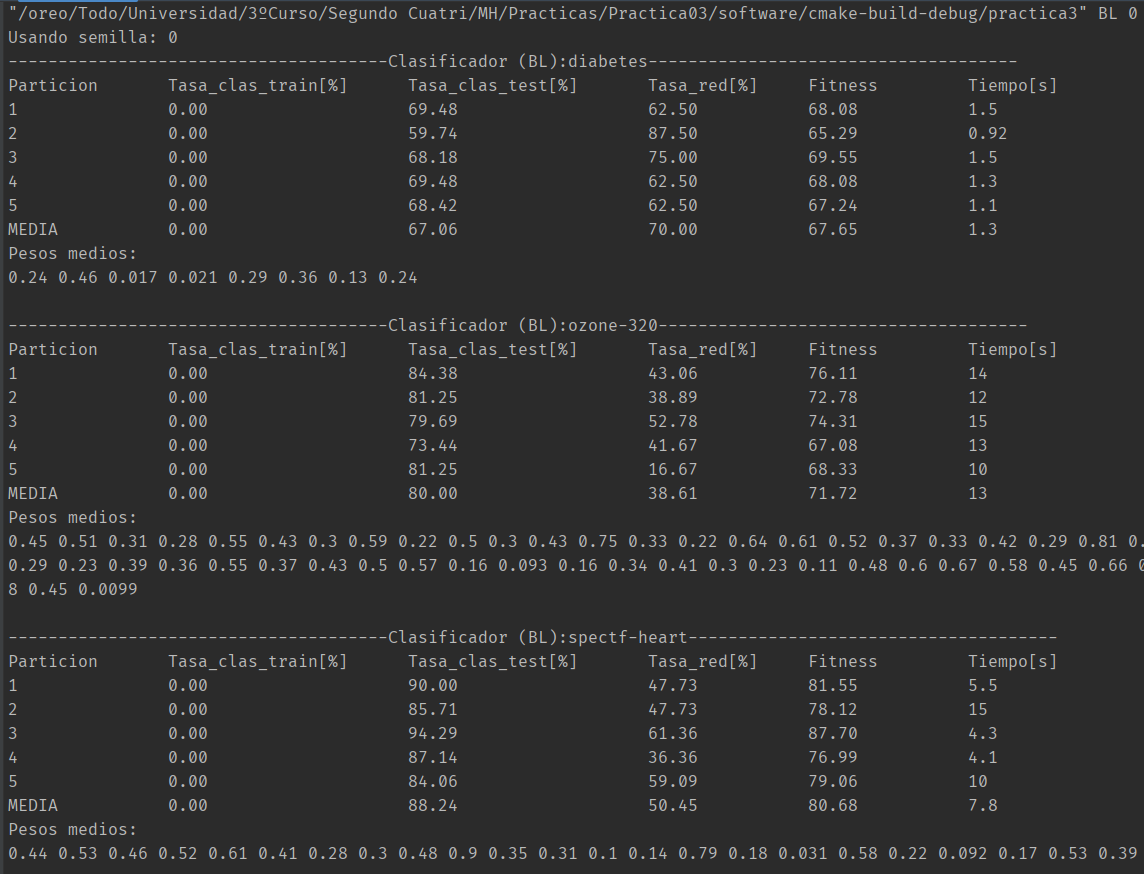
\includegraphics[width=0.75\textwidth]{bl.png}
	\caption{Ejecución de BL}
	\label{fig:greedy}
\end{figure}
Nota: Se añade la tasa\_clas de entrenamiento para comparar en la web. Se puede desactivar quitando el parámetro \code{true} en la linea 142 en main.cpp. Para la ejecución de las tablas siguientes se ha desactivado para mejorar los tiempos. 
\end{itemize}


\subsection{Resultados algoritmos de búsqueda}
Las tablas que se presentan a continuación corresponden a resultados obtenidos por seis algoritmos (BL, BMB, ILS, VNS, ES, ILS-ES) aplicados al problema del Aprendizaje de Pesos en Características (APC) en tres conjuntos de datos diferentes (Diabetes, Ozone y Spectf-heart). Cada tabla muestra los porcentajes de clasificación, reducción del número de características, fitness y tiempo de ejecución para cada partición del conjunto de datos. Se busca comparar la eficacia de ambos algoritmos en términos de calidad de la solución y tiempo de ejecución.

% Please add the following required packages to your document preamble:
% \usepackage{multirow}
% \usepackage[table,xcdraw]{xcolor}
% If you use beamer only pass "xcolor=table" option, i.e. \documentclass[xcolor=table]{beamer}
\begin{table}[H]
	\centering
	\caption{Resultados obtenidos por el algoritmo BL en el problema del APC												
	}
	\label{tab:bl}
	\resizebox{\textwidth}{!}{%
	\begin{tabular}{ccccccccccccc}
		\cline{2-13}
		&
		\multicolumn{4}{c}{\cellcolor[HTML]{C0C0C0}\textbf{Diabetes}} &
		\multicolumn{4}{c}{\cellcolor[HTML]{C0C0C0}\textbf{Ozone}} &
		\multicolumn{4}{c}{\cellcolor[HTML]{C0C0C0}\textbf{Spectf-heart}} \\ \cline{2-13} 
		\multirow{-2}{*}{} &
		\cellcolor[HTML]{DAE8FC}\textit{\textbf{\%\_clas}} &
		\cellcolor[HTML]{DAE8FC}\textit{\textbf{\%\_red}} &
		\cellcolor[HTML]{DAE8FC}\textit{\textbf{Fit.}} &
		\multicolumn{1}{c|}{\cellcolor[HTML]{DAE8FC}\textbf{T}} &
		\cellcolor[HTML]{DAE8FC}\textit{\textbf{\%\_clas}} &
		\cellcolor[HTML]{DAE8FC}\textit{\textbf{\%\_red}} &
		\cellcolor[HTML]{DAE8FC}\textit{\textbf{Fit.}} &
		\multicolumn{1}{c|}{\cellcolor[HTML]{DAE8FC}\textbf{T}} &
		\cellcolor[HTML]{DAE8FC}\textit{\textbf{\%\_clas}} &
		\cellcolor[HTML]{DAE8FC}\textit{\textbf{\%\_red}} &
		\cellcolor[HTML]{DAE8FC}\textit{\textbf{Fit.}} &
		\cellcolor[HTML]{DAE8FC}\textbf{T} \\ \cline{2-13} 
		\multicolumn{1}{c|}{\cellcolor[HTML]{C0C0C0}\textbf{1}} &
		\multicolumn{1}{c|}{70.78} &
		\multicolumn{1}{c|}{62.50} &
		\multicolumn{1}{c|}{69.12} &
		\multicolumn{1}{c|}{6.4} &
		\multicolumn{1}{c|}{76.56} &
		\multicolumn{1}{c|}{15.28} &
		\multicolumn{1}{c|}{64.31} &
		\multicolumn{1}{c|}{22} &
		\multicolumn{1}{c|}{72.86} &
		\multicolumn{1}{c|}{52.27} &
		\multicolumn{1}{c|}{68.74} &
		\multicolumn{1}{c|}{15} \\ \cline{2-13} 
		\multicolumn{1}{c|}{\cellcolor[HTML]{C0C0C0}\textbf{2}} &
		\multicolumn{1}{c|}{72.08} &
		\multicolumn{1}{c|}{62.50} &
		\multicolumn{1}{c|}{70.16} &
		\multicolumn{1}{c|}{13} &
		\multicolumn{1}{c|}{84.38} &
		\multicolumn{1}{c|}{48.61} &
		\multicolumn{1}{c|}{77.22} &
		\multicolumn{1}{c|}{47} &
		\multicolumn{1}{c|}{85.71} &
		\multicolumn{1}{c|}{45.45} &
		\multicolumn{1}{c|}{77.66} &
		\multicolumn{1}{c|}{16} \\ \cline{2-13} 
		\multicolumn{1}{c|}{\cellcolor[HTML]{C0C0C0}\textbf{3}} &
		\multicolumn{1}{c|}{68.18} &
		\multicolumn{1}{c|}{75.00} &
		\multicolumn{1}{c|}{69.55} &
		\multicolumn{1}{c|}{18} &
		\multicolumn{1}{c|}{78.12} &
		\multicolumn{1}{c|}{43.06} &
		\multicolumn{1}{c|}{71.11} &
		\multicolumn{1}{c|}{37} &
		\multicolumn{1}{c|}{90.00} &
		\multicolumn{1}{c|}{34.09} &
		\multicolumn{1}{c|}{78.82} &
		\multicolumn{1}{c|}{11} \\ \cline{2-13} 
		\multicolumn{1}{c|}{\cellcolor[HTML]{C0C0C0}\textbf{4}} &
		\multicolumn{1}{c|}{63.64} &
		\multicolumn{1}{c|}{75.00} &
		\multicolumn{1}{c|}{65.91} &
		\multicolumn{1}{c|}{15} &
		\multicolumn{1}{c|}{70.31} &
		\multicolumn{1}{c|}{43.06} &
		\multicolumn{1}{c|}{64.86} &
		\multicolumn{1}{c|}{24} &
		\multicolumn{1}{c|}{82.86} &
		\multicolumn{1}{c|}{70.45} &
		\multicolumn{1}{c|}{80.38} &
		\multicolumn{1}{c|}{18} \\ \cline{2-13} 
		\multicolumn{1}{c|}{\cellcolor[HTML]{C0C0C0}\textbf{5}} &
		\multicolumn{1}{c|}{71.71} &
		\multicolumn{1}{c|}{75.00} &
		\multicolumn{1}{c|}{72.37} &
		\multicolumn{1}{c|}{6.1} &
		\multicolumn{1}{c|}{82.81} &
		\multicolumn{1}{c|}{47.22} &
		\multicolumn{1}{c|}{75.69} &
		\multicolumn{1}{c|}{30} &
		\multicolumn{1}{c|}{81.16} &
		\multicolumn{1}{c|}{59.09} &
		\multicolumn{1}{c|}{76.75} &
		\multicolumn{1}{c|}{15} \\ \cline{2-13} 
		\multicolumn{1}{c|}{\cellcolor[HTML]{FFFE65}\textbf{M}} &
		\multicolumn{1}{c|}{\textbf{69.28}} &
		\multicolumn{1}{c|}{\textbf{70.00}} &
		\multicolumn{1}{c|}{\textbf{69.42}} &
		\multicolumn{1}{c|}{\textbf{12}} &
		\multicolumn{1}{c|}{\textbf{78.44}} &
		\multicolumn{1}{c|}{\textbf{39.44}} &
		\multicolumn{1}{c|}{\textbf{70.64}} &
		\multicolumn{1}{c|}{\textbf{32}} &
		\multicolumn{1}{c|}{\textbf{82.52}} &
		\multicolumn{1}{c|}{\textbf{52.27}} &
		\multicolumn{1}{c|}{\textbf{76.47}} &
		\multicolumn{1}{c|}{\textbf{15}} \\ \cline{2-13} 
	\end{tabular}
}
\end{table}
La búsqueda local es un enfoque determinista y su rendimiento depende en gran medida de la calidad de la solución inicial y de la exploración del espacio de búsqueda local. Si la solución inicial está cerca de una solución óptima local, la búsqueda local puede converger rápidamente a una solución de alta calidad. Sin embargo, existe el riesgo de quedarse atrapado en óptimos locales y no explorar soluciones mejores en regiones distantes del espacio de búsqueda.\\

En comparación con otros algoritmos, como BMB (Búsqueda Multiarranque Básica), ILS (Búsqueda Local Iterativa), VNS (Variable Neighborhood Search), ES (Enfriamiento Simulado) e ILS-ES (Búsqueda Local Iterativa + Enfriamiento Simulado), la búsqueda local tiene la ventaja de ser simple y fácil de implementar. Sin embargo, puede ser más propensa a quedar atrapada en óptimos locales y puede no ser tan eficiente en la exploración global del espacio de búsqueda. Los otros algoritmos mencionados utilizan estrategias adicionales, como la diversificación de soluciones y la exploración de múltiples vecindarios, para superar esta limitación y buscar soluciones de mayor calidad.\\

De los resultados tendremos en cuenta principalmente el rendimiento medio de la búsqueda local:
\begin{itemize}
	\item clasificación: la clasificación obtenida por la BL es de 69.66, 79.69 y 84.51 en cada dataset de diabetes, ozone y spect-heart respectivamente. Veremos que tan bien clasifican los algoritmos de trayectoria.
	\item Reducción: la reducción obtenida por la BL es de 65\%, 35.83\% y 46.82\% para cada dataset respectivamente. Comprobaremos si reducen más o menos los algoritmos de trayectoria.
	\item Fitness: el fitness obtenido por la BL es de 68.23, 71.31 y 77.25 respectivamente. En los siguientes resultados se comprobará si son mejores o peores resultados.
	\item Tiempo: observaremos como el tiempo de ejecución de la BL es la más baja frente a todos los demás algoritmos. Es lógica ya que el resto se dedican a explorar más el dominio del problema mediante sucesiones de iteraciones de algoritmos de búsqueda.
\end{itemize}

\subsection{Resultados Algoritmos de Trayectoria}

% Please add the following required packages to your document preamble:
% \usepackage{graphicx}
% \usepackage[table,xcdraw]{xcolor}
% If you use beamer only pass "xcolor=table" option, i.e. \documentclass[xcolor=table]{beamer}
\begin{table}[H]
	\centering
	\caption{Resultados obtenidos por la BMB en el problema del APC}
	\label{tab:bmb}
	\resizebox{\textwidth}{!}{%
		\begin{tabular}{c|cccc|cccc|cccc|}
			\cline{2-13}
			\multicolumn{1}{l|}{\textbf{}} &
			\multicolumn{4}{c|}{\textbf{Diabetes}} &
			\multicolumn{4}{c|}{\textbf{Ozone}} &
			\multicolumn{4}{c|}{\textbf{Spectf-heart}} \\ \cline{2-13} 
			\multicolumn{1}{l|}{\textbf{}} &
			\multicolumn{1}{c|}{\textbf{\%\_clas}} &
			\multicolumn{1}{c|}{\textbf{\%\_red}} &
			\multicolumn{1}{c|}{\textbf{Fit.}} &
			\textbf{T{[}s{]}} &
			\multicolumn{1}{c|}{\textbf{\%\_clas}} &
			\multicolumn{1}{c|}{\textbf{\%\_red}} &
			\multicolumn{1}{c|}{\textbf{Fit.}} &
			\textbf{T{[}s{]}} &
			\multicolumn{1}{c|}{\textbf{\%\_clas}} &
			\multicolumn{1}{c|}{\textbf{\%\_red}} &
			\multicolumn{1}{c|}{\textbf{Fit.}} &
			\textbf{T{[}s{]}} \\ \hline
			\multicolumn{1}{|c|}{\textbf{1}} &
			\multicolumn{1}{c|}{70.13} &
			\multicolumn{1}{c|}{62.50} &
			\multicolumn{1}{c|}{68.60} &
			20 &
			\multicolumn{1}{c|}{79.69} &
			\multicolumn{1}{c|}{41.67} &
			\multicolumn{1}{c|}{72.08} &
			87 &
			\multicolumn{1}{c|}{80.00} &
			\multicolumn{1}{c|}{68.18} &
			\multicolumn{1}{c|}{77.64} &
			53 \\ \hline
			\multicolumn{1}{|c|}{\textbf{2}} &
			\multicolumn{1}{c|}{65.58} &
			\multicolumn{1}{c|}{62.50} &
			\multicolumn{1}{c|}{64.97} &
			24 &
			\multicolumn{1}{c|}{76.56} &
			\multicolumn{1}{c|}{48.61} &
			\multicolumn{1}{c|}{70.97} &
			69 &
			\multicolumn{1}{c|}{90.00} &
			\multicolumn{1}{c|}{61.36} &
			\multicolumn{1}{c|}{84.27} &
			60 \\ \hline
			\multicolumn{1}{|c|}{\textbf{3}} &
			\multicolumn{1}{c|}{66.88} &
			\multicolumn{1}{c|}{62.50} &
			\multicolumn{1}{c|}{66.01} &
			22 &
			\multicolumn{1}{c|}{79.69} &
			\multicolumn{1}{c|}{50.00} &
			\multicolumn{1}{c|}{73.75} &
			77 &
			\multicolumn{1}{c|}{87.14} &
			\multicolumn{1}{c|}{54.55} &
			\multicolumn{1}{c|}{80.62} &
			65 \\ \hline
			\multicolumn{1}{|c|}{\textbf{4}} &
			\multicolumn{1}{c|}{63.64} &
			\multicolumn{1}{c|}{75.00} &
			\multicolumn{1}{c|}{65.91} &
			21 &
			\multicolumn{1}{c|}{78.12} &
			\multicolumn{1}{c|}{50.00} &
			\multicolumn{1}{c|}{72.50} &
			62 &
			\multicolumn{1}{c|}{80.00} &
			\multicolumn{1}{c|}{61.36} &
			\multicolumn{1}{c|}{76.27} &
			52 \\ \hline
			\multicolumn{1}{|c|}{\textbf{5}} &
			\multicolumn{1}{c|}{69.74} &
			\multicolumn{1}{c|}{75.00} &
			\multicolumn{1}{c|}{70.79} &
			23 &
			\multicolumn{1}{c|}{78.12} &
			\multicolumn{1}{c|}{43.06} &
			\multicolumn{1}{c|}{71.11} &
			63 &
			\multicolumn{1}{c|}{86.96} &
			\multicolumn{1}{c|}{68.18} &
			\multicolumn{1}{c|}{83.20} &
			49 \\ \hline
			\multicolumn{1}{|c|}{{\color[HTML]{00009B} \textbf{M}}} &
			\multicolumn{1}{c|}{{\color[HTML]{00009B} \textbf{67.19}}} &
			\multicolumn{1}{c|}{{\color[HTML]{00009B} \textbf{67.50}}} &
			\multicolumn{1}{c|}{{\color[HTML]{00009B} \textbf{67.26}}} &
			{\color[HTML]{00009B} \textbf{22}} &
			\multicolumn{1}{c|}{{\color[HTML]{00009B} \textbf{78.44}}} &
			\multicolumn{1}{c|}{{\color[HTML]{00009B} \textbf{46.67}}} &
			\multicolumn{1}{c|}{{\color[HTML]{00009B} \textbf{72.08}}} &
			{\color[HTML]{00009B} \textbf{72}} &
			\multicolumn{1}{c|}{{\color[HTML]{00009B} \textbf{84.82}}} &
			\multicolumn{1}{c|}{{\color[HTML]{00009B} \textbf{62.73}}} &
			\multicolumn{1}{c|}{{\color[HTML]{00009B} \textbf{80.40}}} &
			{\color[HTML]{00009B} \textbf{56}} \\ \hline
		\end{tabular}%
	}
\end{table}
Vamos a comparar los resultados con la Búsqueda Local en función de cada dataset:

\begin{enumerate}
\item Diabetes: 
\begin{itemize}
\item BL tiene un mejor rendimiento en términos de porcentaje de clasificación (69.66\%) en comparación con BMB (67.19\%).
\item Ambos algoritmos obtienen el mismo porcentaje de reducción de 62.50\%.
\item BL obtiene un mejor fitness (68.23) en comparación con BMB (67.26).
\item BL es considerablemente más rápido en términos de tiempo de ejecución, requiriendo solo 1.8 segundos en promedio, mientras que BMB requiere 22 segundos.
\end{itemize}

\item Ozone:
\begin{itemize}
\item BL muestra un mejor rendimiento en términos de porcentaje de clasificación (79.69\%) en comparación con BMB (78.44\%).
\item BMB logra una mayor reducción en el número de características utilizadas, con un porcentaje de reducción promedio de 46.67\%, mientras que BL logra 37.78\%.
\item BMB obtiene un mejor fitness (72.08) en comparación con BL (71.31).
\item BL es más rápido en términos de tiempo de ejecución, requiriendo 16 segundos en promedio, mientras que BMB requiere 72 segundos.
\end{itemize}

\item Spectf-heart:
\begin{itemize}
	\item Ambos algoritmos obtienen resultados de clasificación similares, con BL y BMB alcanzando un porcentaje de clasificación promedio de 84.51\% y 84.82\%, respectivamente.
	\item BMB logra una mayor reducción en el número de características utilizadas, con un porcentaje de reducción promedio de 62.73\%, mientras que BL logra 48.18\%.
	\item BMB obtiene un mejor fitness (80.40) en comparación con BL (77.25).
	\item BL es más rápido en términos de tiempo de ejecución, requiriendo 6.3 segundos en promedio, mientras que BMB requiere 56 segundos.
\end{itemize}

\end{enumerate}

Resumidamente, al menos según los resultados, la Búsqueda Local (BL) muestra un mejor rendimiento en términos de clasificación y tiempo de ejecución en los conjuntos de datos Diabetes y Ozone. Lo cual tiene sentido ya que estamos ejecutando 15 veces la búsqueda local, aumentando el tiempo sensiblemente. Sin embargo, en el conjunto de datos Spectf-heart, aunque BL es más rápido, Búsqueda Multiarranque Básica (BMB) obtiene un mejor fitness y logra una mayor reducción en el número de características utilizadas.

% Please add the following required packages to your document preamble:
% \usepackage{graphicx}
% \usepackage[table,xcdraw]{xcolor}
% If you use beamer only pass "xcolor=table" option, i.e. \documentclass[xcolor=table]{beamer}
\begin{table}[H]
	\centering
	\caption{Resultados obtenidos por el algoritmo ILS en el problema del APC}
	\label{tab:ILS}
	\resizebox{\textwidth}{!}{%
		\begin{tabular}{c|cccc|cccc|cccc|}
			\cline{2-13}
			\multicolumn{1}{l|}{} &
			\multicolumn{4}{c|}{\textbf{Diabetes}} &
			\multicolumn{4}{c|}{\textbf{Ozone}} &
			\multicolumn{4}{c|}{\textbf{Spectf-heart}} \\ \cline{2-13} 
			\multicolumn{1}{l|}{} &
			\multicolumn{1}{c|}{\textbf{\%\_clas}} &
			\multicolumn{1}{c|}{\textbf{\%\_red}} &
			\multicolumn{1}{c|}{\textbf{Fit.}} &
			\textbf{T{[}s{]}} &
			\multicolumn{1}{c|}{\textbf{\%\_clas}} &
			\multicolumn{1}{c|}{\textbf{\%\_red}} &
			\multicolumn{1}{c|}{\textbf{Fit.}} &
			\textbf{T{[}s{]}} &
			\multicolumn{1}{c|}{\textbf{\%\_clas}} &
			\multicolumn{1}{c|}{\textbf{\%\_red}} &
			\multicolumn{1}{c|}{\textbf{Fit.}} &
			\textbf{T{[}s{]}} \\ \hline
			\multicolumn{1}{|c|}{\textbf{1}} &
			\multicolumn{1}{c|}{69.48} &
			\multicolumn{1}{c|}{62.50} &
			\multicolumn{1}{c|}{68.08} &
			16 &
			\multicolumn{1}{c|}{79.69} &
			\multicolumn{1}{c|}{56.94} &
			\multicolumn{1}{c|}{75.14} &
			95 &
			\multicolumn{1}{c|}{84.29} &
			\multicolumn{1}{c|}{63.64} &
			\multicolumn{1}{c|}{80.16} &
			55 \\ \hline
			\multicolumn{1}{|c|}{\textbf{2}} &
			\multicolumn{1}{c|}{72.08} &
			\multicolumn{1}{c|}{62.50} &
			\multicolumn{1}{c|}{70.16} &
			19 &
			\multicolumn{1}{c|}{82.81} &
			\multicolumn{1}{c|}{52.78} &
			\multicolumn{1}{c|}{76.81} &
			88 &
			\multicolumn{1}{c|}{80.00} &
			\multicolumn{1}{c|}{70.45} &
			\multicolumn{1}{c|}{78.09} &
			57 \\ \hline
			\multicolumn{1}{|c|}{\textbf{3}} &
			\multicolumn{1}{c|}{66.88} &
			\multicolumn{1}{c|}{62.50} &
			\multicolumn{1}{c|}{66.01} &
			23 &
			\multicolumn{1}{c|}{85.94} &
			\multicolumn{1}{c|}{51.39} &
			\multicolumn{1}{c|}{79.03} &
			87 &
			\multicolumn{1}{c|}{92.86} &
			\multicolumn{1}{c|}{70.45} &
			\multicolumn{1}{c|}{88.38} &
			60 \\ \hline
			\multicolumn{1}{|c|}{\textbf{4}} &
			\multicolumn{1}{c|}{63.64} &
			\multicolumn{1}{c|}{75.00} &
			\multicolumn{1}{c|}{65.91} &
			20 &
			\multicolumn{1}{c|}{70.31} &
			\multicolumn{1}{c|}{51.39} &
			\multicolumn{1}{c|}{66.53} &
			88 &
			\multicolumn{1}{c|}{81.43} &
			\multicolumn{1}{c|}{63.64} &
			\multicolumn{1}{c|}{77.87} &
			56 \\ \hline
			\multicolumn{1}{|c|}{\textbf{5}} &
			\multicolumn{1}{c|}{69.74} &
			\multicolumn{1}{c|}{75.00} &
			\multicolumn{1}{c|}{70.79} &
			22 &
			\multicolumn{1}{c|}{85.94} &
			\multicolumn{1}{c|}{47.22} &
			\multicolumn{1}{c|}{78.19} &
			86 &
			\multicolumn{1}{c|}{81.16} &
			\multicolumn{1}{c|}{63.64} &
			\multicolumn{1}{c|}{77.65} &
			64 \\ \hline
			\multicolumn{1}{|c|}{{\color[HTML]{00009B} \textbf{M}}} &
			\multicolumn{1}{c|}{{\color[HTML]{00009B} \textbf{68.36}}} &
			\multicolumn{1}{c|}{{\color[HTML]{00009B} \textbf{67.50}}} &
			\multicolumn{1}{c|}{{\color[HTML]{00009B} \textbf{68.19}}} &
			{\color[HTML]{00009B} \textbf{20}} &
			\multicolumn{1}{c|}{{\color[HTML]{00009B} \textbf{80.94}}} &
			\multicolumn{1}{c|}{{\color[HTML]{00009B} \textbf{51.94}}} &
			\multicolumn{1}{c|}{{\color[HTML]{00009B} \textbf{75.14}}} &
			{\color[HTML]{00009B} \textbf{89}} &
			\multicolumn{1}{c|}{{\color[HTML]{00009B} \textbf{83.95}}} &
			\multicolumn{1}{c|}{{\color[HTML]{00009B} \textbf{66.36}}} &
			\multicolumn{1}{c|}{{\color[HTML]{00009B} \textbf{80.43}}} &
			{\color[HTML]{00009B} \textbf{58}} \\ \hline
		\end{tabular}%
	}
\end{table}

Al comparar los resultados de Búsqueda Local (BL) y Búsqueda Local Iterada (ILS) en los diferentes conjuntos de datos, podemos observar lo siguiente:

\begin{enumerate}
	
\item Diabetes:

\begin{itemize}
\item BL tiene un mejor rendimiento en términos de porcentaje de clasificación (69.66\%) en comparación con ILS (68.36\%).
\item  ILS reduce un 5\% más que la BL (67.50\% vs 62.50\%).
\item  Ambos algoritmos obtienen un fitness muy similar (68.23).
\item  ILS es sensiblemente más lento en términos de tiempo de ejecución, requiriendo 20 segundos en promedio, mientras que BL requiere 1.8 segundos. Es lógico ya que se llama 15 veces a la búsqueda local.
\end{itemize}

\item Ozone:

\begin{itemize}
	\item ILS muestra un mejor rendimiento en términos de porcentaje de clasificación (80.94\%) en comparación con BL (79.69\%).
 \item ILS logra una mayor reducción en el número de características utilizadas, con un porcentaje de reducción promedio de 51.94\%, mientras que BL logra 37.78\%.
 \item ILS obtiene un mejor fitness (75.14) en comparación con BL (71.31).
 \item BL es más rápido en términos de tiempo de ejecución, requiriendo 16 segundos en promedio, mientras que ILS requiere 89 segundos.
\end{itemize}

\item Spectf-heart:

\begin{itemize}
	\item BL muestra un mejor rendimiento en términos de porcentaje de clasificación (84.51\%)en comparación con ILS (83.95\%).

 \item ILS logra una mayor reducción en el número de características utilizadas, con un porcentaje de reducción promedio de 66.36\%, mientras que BL logra 48.18\%.

\item  ILS obtiene un mejor fitness (80.43) en comparación con BL (77.25).

\item  BL es más rápido en términos de tiempo de ejecución, requiriendo 6.3 segundos en promedio, mientras que ILS requiere 58 segundos.
\end{itemize}
Según los resultados obtenidos, la Búsqueda Local Iterada (ILS) muestra un mejor rendimiento en términos de clasificación en los conjuntos de datos Ozone y Spectf-heart, mientras que la Búsqueda Local (BL) es mejor en el conjunto de datos Diabetes. Sin embargo, BL es más rápida en términos de tiempo de ejecución en todos los conjuntos de datos. ILS logra una mayor reducción y mejores fitness en los conjuntos de datos Ozone y Spectf-heart.

\end{enumerate}

% Please add the following required packages to your document preamble:
% \usepackage{graphicx}
% \usepackage[table,xcdraw]{xcolor}
% If you use beamer only pass "xcolor=table" option, i.e. \documentclass[xcolor=table]{beamer}
\begin{table}[H]
	\centering
	\caption{Resultados obtenidos por el algoritmo VNS en el problema del APC}
	\label{tab:VNS}
	\resizebox{\textwidth}{!}{%
		\begin{tabular}{c|cccc|cccc|cccc|}
			\cline{2-13}
			\multicolumn{1}{l|}{} &
			\multicolumn{4}{c|}{\textbf{Diabetes}} &
			\multicolumn{4}{c|}{\textbf{Ozone}} &
			\multicolumn{4}{c|}{\textbf{Spectf-heart}} \\ \cline{2-13} 
			\multicolumn{1}{l|}{} &
			\multicolumn{1}{c|}{\textbf{\%\_clas}} &
			\multicolumn{1}{c|}{\textbf{\%\_red}} &
			\multicolumn{1}{c|}{\textbf{Fit.}} &
			\textbf{T{[}s{]}} &
			\multicolumn{1}{c|}{\textbf{\%\_clas}} &
			\multicolumn{1}{c|}{\textbf{\%\_red}} &
			\multicolumn{1}{c|}{\textbf{Fit.}} &
			\textbf{T{[}s{]}} &
			\multicolumn{1}{c|}{\textbf{\%\_clas}} &
			\multicolumn{1}{c|}{\textbf{\%\_red}} &
			\multicolumn{1}{c|}{\textbf{Fit.}} &
			\textbf{T{[}s{]}} \\ \hline
			\multicolumn{1}{|c|}{\textbf{1}} &
			\multicolumn{1}{c|}{64.94} &
			\multicolumn{1}{c|}{100.00} &
			\multicolumn{1}{c|}{71.95} &
			20 &
			\multicolumn{1}{c|}{79.69} &
			\multicolumn{1}{c|}{51.39} &
			\multicolumn{1}{c|}{74.03} &
			83 &
			\multicolumn{1}{c|}{87.14} &
			\multicolumn{1}{c|}{54.55} &
			\multicolumn{1}{c|}{80.62} &
			53 \\ \hline
			\multicolumn{1}{|c|}{\textbf{2}} &
			\multicolumn{1}{c|}{67.53} &
			\multicolumn{1}{c|}{62.50} &
			\multicolumn{1}{c|}{66.53} &
			25 &
			\multicolumn{1}{c|}{78.12} &
			\multicolumn{1}{c|}{44.44} &
			\multicolumn{1}{c|}{71.39} &
			88 &
			\multicolumn{1}{c|}{87.14} &
			\multicolumn{1}{c|}{61.36} &
			\multicolumn{1}{c|}{81.99} &
			56 \\ \hline
			\multicolumn{1}{|c|}{\textbf{3}} &
			\multicolumn{1}{c|}{66.88} &
			\multicolumn{1}{c|}{62.50} &
			\multicolumn{1}{c|}{66.01} &
			30 &
			\multicolumn{1}{c|}{76.56} &
			\multicolumn{1}{c|}{47.22} &
			\multicolumn{1}{c|}{70.69} &
			85 &
			\multicolumn{1}{c|}{85.71} &
			\multicolumn{1}{c|}{43.18} &
			\multicolumn{1}{c|}{77.21} &
			57 \\ \hline
			\multicolumn{1}{|c|}{\textbf{4}} &
			\multicolumn{1}{c|}{63.64} &
			\multicolumn{1}{c|}{75.00} &
			\multicolumn{1}{c|}{65.91} &
			19 &
			\multicolumn{1}{c|}{75.00} &
			\multicolumn{1}{c|}{45.83} &
			\multicolumn{1}{c|}{69.17} &
			86 &
			\multicolumn{1}{c|}{82.86} &
			\multicolumn{1}{c|}{54.55} &
			\multicolumn{1}{c|}{77.19} &
			51 \\ \hline
			\multicolumn{1}{|c|}{\textbf{5}} &
			\multicolumn{1}{c|}{69.74} &
			\multicolumn{1}{c|}{75.00} &
			\multicolumn{1}{c|}{70.79} &
			20 &
			\multicolumn{1}{c|}{84.38} &
			\multicolumn{1}{c|}{36.11} &
			\multicolumn{1}{c|}{74.72} &
			93 &
			\multicolumn{1}{c|}{84.06} &
			\multicolumn{1}{c|}{43.18} &
			\multicolumn{1}{c|}{75.88} &
			60 \\ \hline
			\multicolumn{1}{|c|}{{\color[HTML]{00009B} \textbf{M}}} &
			\multicolumn{1}{c|}{{\color[HTML]{00009B} \textbf{66.54}}} &
			\multicolumn{1}{c|}{{\color[HTML]{00009B} \textbf{75.00}}} &
			\multicolumn{1}{c|}{{\color[HTML]{00009B} \textbf{68.24}}} &
			{\color[HTML]{00009B} \textbf{23}} &
			\multicolumn{1}{c|}{{\color[HTML]{00009B} \textbf{78.75}}} &
			\multicolumn{1}{c|}{{\color[HTML]{00009B} \textbf{45.00}}} &
			\multicolumn{1}{c|}{{\color[HTML]{00009B} \textbf{72.00}}} &
			{\color[HTML]{00009B} \textbf{87}} &
			\multicolumn{1}{c|}{{\color[HTML]{00009B} \textbf{85.38}}} &
			\multicolumn{1}{c|}{{\color[HTML]{00009B} \textbf{51.36}}} &
			\multicolumn{1}{c|}{{\color[HTML]{00009B} \textbf{78.58}}} &
			{\color[HTML]{00009B} \textbf{56}} \\ \hline
		\end{tabular}%
	}
\end{table}
Al comparar los resultados de Búsqueda Local (BL) y Búsqueda por Vecindarios Variables (VNS) en los diferentes conjuntos de datos, podemos observar lo siguiente:

\begin{enumerate}
\item Diabetes:
\begin{itemize}
\item	BL obtiene un porcentaje de clasificación mejor (69.66\%) en comparación con VNS (66.54\%).
\item	VNS logra una reducción del 75.00\% en el número de características utilizadas, mientras que BL logra 62.50\%.
\item	Ambos algoritmos tienen prácticamente el mismo fitness (68.23).
\item	VNS es más lento en términos de tiempo de ejecución, requiriendo 23 segundos en promedio, mientras que BL requiere 1.8 segundos.
\end{itemize}

\item Ozone:
\begin{itemize}
\item BL muestra un mejor rendimiento en términos de porcentaje de clasificación (79.69\%) en comparación con VNS (78.75\%).
\item VNS logra una mayor reducción en el número de características utilizadas, con un porcentaje de reducción promedio de 45.00\%, mientras que BL logra 37.78\%.
\item VNS obtiene un ligeramente mejor fitness (72.00) en comparación con BL (71.31).
\item BL es más rápido en términos de tiempo de ejecución, requiriendo 16 segundos en promedio, mientras que VNS requiere 87 segundos.
\end{itemize}


\item Spectf-heart:
\begin{itemize}
\item VNS muestra un mejor rendimiento en términos de porcentaje de clasificación (85.38\%) en comparación con BL (84.51\%).
\item VNS logra una mayor reducción en el número de características utilizadas, con un porcentaje de reducción promedio de 51.36\%, mientras que BL logra 48.18\%.
\item VNS obtiene un mejor fitness (78.58) en comparación con BL (77.25).
\item BL es más rápido en términos de tiempo de ejecución, requiriendo 6.3 segundos en promedio, mientras que VNS requiere 56 segundos.
\end{itemize}

\end{enumerate}

Resumidamente, la Búsqueda Local (BL) muestra un mejor rendimiento en términos de clasificación en los conjuntos de datos Diabetes y Ozone, mientras que la Búsqueda por Vecindarios Variables (VNS) es mejor en el conjunto de datos Spectf-heart. Sin embargo, BL es más rápida en términos de tiempo de ejecución en todos los conjuntos de datos. VNS logra una mayor reducción y mejores fitness en los conjuntos de datos Ozone y Spectf-heart.

% Please add the following required packages to your document preamble:
% \usepackage{graphicx}
% \usepackage[table,xcdraw]{xcolor}
% If you use beamer only pass "xcolor=table" option, i.e. \documentclass[xcolor=table]{beamer}
\begin{table}[H]
	\centering
	\caption{Resultados obtenidos por el algoritmo ES en el problema del APC}
	\label{tab:ES}
	\resizebox{\textwidth}{!}{%
		\begin{tabular}{c|cccc|cccc|cccc|}
			\cline{2-13}
			\multicolumn{1}{l|}{} &
			\multicolumn{4}{c|}{\textbf{Diabetes}} &
			\multicolumn{4}{c|}{\textbf{Ozone}} &
			\multicolumn{4}{c|}{\textbf{Spectf-heart}} \\ \cline{2-13} 
			\multicolumn{1}{l|}{} &
			\multicolumn{1}{c|}{\textbf{\%\_clas}} &
			\multicolumn{1}{c|}{\textbf{\%\_red}} &
			\multicolumn{1}{c|}{\textbf{Fit.}} &
			\textbf{T{[}s{]}} &
			\multicolumn{1}{c|}{\textbf{\%\_clas}} &
			\multicolumn{1}{c|}{\textbf{\%\_red}} &
			\multicolumn{1}{c|}{\textbf{Fit.}} &
			\textbf{T{[}s{]}} &
			\multicolumn{1}{c|}{\textbf{\%\_clas}} &
			\multicolumn{1}{c|}{\textbf{\%\_red}} &
			\multicolumn{1}{c|}{\textbf{Fit.}} &
			\textbf{T{[}s{]}} \\ \hline
			\multicolumn{1}{|c|}{\textbf{1}} &
			\multicolumn{1}{c|}{69.48} &
			\multicolumn{1}{c|}{62.50} &
			\multicolumn{1}{c|}{68.08} &
			65 &
			\multicolumn{1}{c|}{75.00} &
			\multicolumn{1}{c|}{58.33} &
			\multicolumn{1}{c|}{71.67} &
			80 &
			\multicolumn{1}{c|}{80.00} &
			\multicolumn{1}{c|}{59.09} &
			\multicolumn{1}{c|}{75.82} &
			64 \\ \hline
			\multicolumn{1}{|c|}{\textbf{2}} &
			\multicolumn{1}{c|}{67.53} &
			\multicolumn{1}{c|}{62.50} &
			\multicolumn{1}{c|}{66.53} &
			65 &
			\multicolumn{1}{c|}{79.69} &
			\multicolumn{1}{c|}{58.33} &
			\multicolumn{1}{c|}{75.42} &
			85 &
			\multicolumn{1}{c|}{88.57} &
			\multicolumn{1}{c|}{54.55} &
			\multicolumn{1}{c|}{81.77} &
			56 \\ \hline
			\multicolumn{1}{|c|}{\textbf{3}} &
			\multicolumn{1}{c|}{66.88} &
			\multicolumn{1}{c|}{62.50} &
			\multicolumn{1}{c|}{66.01} &
			76 &
			\multicolumn{1}{c|}{79.69} &
			\multicolumn{1}{c|}{63.89} &
			\multicolumn{1}{c|}{76.53} &
			80 &
			\multicolumn{1}{c|}{90.00} &
			\multicolumn{1}{c|}{56.82} &
			\multicolumn{1}{c|}{83.36} &
			58 \\ \hline
			\multicolumn{1}{|c|}{\textbf{4}} &
			\multicolumn{1}{c|}{68.83} &
			\multicolumn{1}{c|}{62.50} &
			\multicolumn{1}{c|}{67.56} &
			72 &
			\multicolumn{1}{c|}{70.31} &
			\multicolumn{1}{c|}{52.78} &
			\multicolumn{1}{c|}{66.81} &
			87 &
			\multicolumn{1}{c|}{84.29} &
			\multicolumn{1}{c|}{61.36} &
			\multicolumn{1}{c|}{79.70} &
			60 \\ \hline
			\multicolumn{1}{|c|}{\textbf{5}} &
			\multicolumn{1}{c|}{69.74} &
			\multicolumn{1}{c|}{75.00} &
			\multicolumn{1}{c|}{70.79} &
			67 &
			\multicolumn{1}{c|}{84.38} &
			\multicolumn{1}{c|}{58.33} &
			\multicolumn{1}{c|}{79.17} &
			79 &
			\multicolumn{1}{c|}{76.81} &
			\multicolumn{1}{c|}{70.45} &
			\multicolumn{1}{c|}{75.54} &
			53 \\ \hline
			\multicolumn{1}{|c|}{{\color[HTML]{00009B} \textbf{M}}} &
			\multicolumn{1}{c|}{{\color[HTML]{00009B} \textbf{68.49}}} &
			\multicolumn{1}{c|}{{\color[HTML]{00009B} \textbf{65.00}}} &
			\multicolumn{1}{c|}{{\color[HTML]{00009B} \textbf{67.79}}} &
			{\color[HTML]{00009B} \textbf{69}} &
			\multicolumn{1}{c|}{{\color[HTML]{00009B} \textbf{77.81}}} &
			\multicolumn{1}{c|}{{\color[HTML]{00009B} \textbf{58.33}}} &
			\multicolumn{1}{c|}{{\color[HTML]{00009B} \textbf{73.92}}} &
			{\color[HTML]{00009B} \textbf{82}} &
			\multicolumn{1}{c|}{{\color[HTML]{00009B} \textbf{83.93}}} &
			\multicolumn{1}{c|}{{\color[HTML]{00009B} \textbf{60.45}}} &
			\multicolumn{1}{c|}{{\color[HTML]{00009B} \textbf{79.24}}} &
			{\color[HTML]{00009B} \textbf{58}} \\ \hline
		\end{tabular}%
	}
\end{table}
Al comparar los resultados de Búsqueda Local (BL) y Enfriamiento Simulado (ES) en los diferentes conjuntos de datos, podemos observar lo siguiente:

\begin{enumerate}
	\item Diabetes:
	\begin{itemize}
\item BL obtiene un porcentaje de clasificación ligeramente mejor (69.66\%) en comparación con ES (68.49\%).
\item  Ambos algoritmos logran la misma reducción en el número de características utilizadas, con un porcentaje de reducción de 62.50\%.
\item BL obtiene un mejor fitness (68.23) en comparación con ES (67.79).
\item BL es más rápido en términos de tiempo de ejecución, requiriendo 1.8 segundos en promedio, mientras que ES requiere 69 segundos.
	\end{itemize}

\item Ozone:
\begin{itemize}
\item BL muestra un mejor rendimiento en términos de porcentaje de clasificación (79.69\%) en comparación con ES (77.81\%).
\item ES logra una reducción del 58.33\% en el número de características utilizadas, mientras que BL se queda una reducción del 37.78\% .
\item ES obtiene un mejor fitness (73.92) en comparación con BL (72.00).
\item BL es más rápido en términos de tiempo de ejecución, requiriendo 16 segundos en promedio, mientras que ES requiere 82 segundos.
\end{itemize}

\item Spectf-heart:
\begin{itemize}
\item BL muestra un mejor rendimiento en términos de porcentaje de clasificación (84.51\%)en comparación con ES (83.93\%).
\item ES consigue una reducción considerablemente mayor (60.45\%) en comparación a BL (48.18\%)
\item ES obtiene un mejor fitness (79.24) en comparación con BL (77.25).
\item BL es más rápido en términos de tiempo de ejecución, requiriendo 6.3 segundos en promedio, mientras que ES requiere 82 segundos.
\end{itemize}

Concluimos que la Búsqueda Local (BL) muestra un mejor rendimiento en términos de clasificación en los conjuntos de datos Diabetes y Ozone, mientras que el Enfriamiento Simulado (ES) es mejor en el conjunto de datos Spectf-heart. BL también es más rápido en tiempo de ejecución en todos los conjuntos de datos. Sin embargo, ES logra una mayor reducción en el número de características utilizadas y mejores fitness en los conjuntos de datos Ozone y Spectf-heart.

\end{enumerate}
% Please add the following required packages to your document preamble:
% \usepackage{graphicx}
% \usepackage[table,xcdraw]{xcolor}
% If you use beamer only pass "xcolor=table" option, i.e. \documentclass[xcolor=table]{beamer}
\begin{table}[H]
	\centering
	\caption{Resultados obtenidos por el algoritmo ILS-ES en el problema del APC}
	\label{tab:ILS-ES}
	\resizebox{\textwidth}{!}{%
		\begin{tabular}{c|cccc|cccc|cccc|}
			\cline{2-13}
			\multicolumn{1}{l|}{} &
			\multicolumn{4}{c|}{\textbf{Diabetes}} &
			\multicolumn{4}{c|}{\textbf{Ozone}} &
			\multicolumn{4}{c|}{\textbf{Spectf-heart}} \\ \cline{2-13} 
			\multicolumn{1}{l|}{} &
			\multicolumn{1}{c|}{\textbf{\%\_clas}} &
			\multicolumn{1}{c|}{\textbf{\%\_red}} &
			\multicolumn{1}{c|}{\textbf{Fit.}} &
			\textbf{T{[}s{]}} &
			\multicolumn{1}{c|}{\textbf{\%\_clas}} &
			\multicolumn{1}{c|}{\textbf{\%\_red}} &
			\multicolumn{1}{c|}{\textbf{Fit.}} &
			\textbf{T{[}s{]}} &
			\multicolumn{1}{c|}{\textbf{\%\_clas}} &
			\multicolumn{1}{c|}{\textbf{\%\_red}} &
			\multicolumn{1}{c|}{\textbf{Fit.}} &
			\textbf{T{[}s{]}} \\ \hline
			\multicolumn{1}{|c|}{\textbf{1}} &
			\multicolumn{1}{c|}{64.94} &
			\multicolumn{1}{c|}{100.00} &
			\multicolumn{1}{c|}{71.95} &
			64 &
			\multicolumn{1}{c|}{78.12} &
			\multicolumn{1}{c|}{56.94} &
			\multicolumn{1}{c|}{73.89} &
			97 &
			\multicolumn{1}{c|}{84.29} &
			\multicolumn{1}{c|}{68.18} &
			\multicolumn{1}{c|}{81.06} &
			69 \\ \hline
			\multicolumn{1}{|c|}{\textbf{2}} &
			\multicolumn{1}{c|}{66.88} &
			\multicolumn{1}{c|}{62.50} &
			\multicolumn{1}{c|}{66.01} &
			72 &
			\multicolumn{1}{c|}{82.81} &
			\multicolumn{1}{c|}{56.94} &
			\multicolumn{1}{c|}{77.64} &
			98 &
			\multicolumn{1}{c|}{87.14} &
			\multicolumn{1}{c|}{75.00} &
			\multicolumn{1}{c|}{84.71} &
			69 \\ \hline
			\multicolumn{1}{|c|}{\textbf{3}} &
			\multicolumn{1}{c|}{66.23} &
			\multicolumn{1}{c|}{62.50} &
			\multicolumn{1}{c|}{65.49} &
			66 &
			\multicolumn{1}{c|}{84.38} &
			\multicolumn{1}{c|}{55.56} &
			\multicolumn{1}{c|}{78.61} &
			86 &
			\multicolumn{1}{c|}{91.43} &
			\multicolumn{1}{c|}{63.64} &
			\multicolumn{1}{c|}{85.87} &
			67 \\ \hline
			\multicolumn{1}{|c|}{\textbf{4}} &
			\multicolumn{1}{c|}{63.64} &
			\multicolumn{1}{c|}{75.00} &
			\multicolumn{1}{c|}{65.91} &
			76 &
			\multicolumn{1}{c|}{76.56} &
			\multicolumn{1}{c|}{55.56} &
			\multicolumn{1}{c|}{72.36} &
			95 &
			\multicolumn{1}{c|}{82.86} &
			\multicolumn{1}{c|}{70.45} &
			\multicolumn{1}{c|}{80.38} &
			68 \\ \hline
			\multicolumn{1}{|c|}{\textbf{5}} &
			\multicolumn{1}{c|}{69.74} &
			\multicolumn{1}{c|}{75.00} &
			\multicolumn{1}{c|}{70.79} &
			76 &
			\multicolumn{1}{c|}{85.94} &
			\multicolumn{1}{c|}{55.56} &
			\multicolumn{1}{c|}{79.86} &
			92 &
			\multicolumn{1}{c|}{84.06} &
			\multicolumn{1}{c|}{70.45} &
			\multicolumn{1}{c|}{81.34} &
			68 \\ \hline
			\multicolumn{1}{|c|}{{\color[HTML]{00009B} \textbf{M}}} &
			\multicolumn{1}{c|}{{\color[HTML]{00009B} \textbf{66.29}}} &
			\multicolumn{1}{c|}{{\color[HTML]{00009B} \textbf{75.00}}} &
			\multicolumn{1}{c|}{{\color[HTML]{00009B} \textbf{68.03}}} &
			{\color[HTML]{00009B} \textbf{71}} &
			\multicolumn{1}{c|}{{\color[HTML]{00009B} \textbf{81.56}}} &
			\multicolumn{1}{c|}{{\color[HTML]{00009B} \textbf{56.11}}} &
			\multicolumn{1}{c|}{{\color[HTML]{00009B} \textbf{76.47}}} &
			{\color[HTML]{00009B} \textbf{94}} &
			\multicolumn{1}{c|}{{\color[HTML]{00009B} \textbf{85.95}}} &
			\multicolumn{1}{c|}{{\color[HTML]{00009B} \textbf{69.55}}} &
			\multicolumn{1}{c|}{{\color[HTML]{00009B} \textbf{82.67}}} &
			{\color[HTML]{00009B} \textbf{68}} \\ \hline
		\end{tabular}%
	}
\end{table}

Al comparar los resultados de Búsqueda Local (BL) y Búsqueda Local Iterada con Enfriamiento Simulado (ILS-ES) en los diferentes conjuntos de datos, podemos observar lo siguiente:

\begin{enumerate}

\item Diabetes:

\begin{itemize}
\item BL obtiene un porcentaje de clasificación ligeramente mejor (69.66\%) en comparación con ILS-ES (66.29\%).
\item ES-ILS consigue una reducción considerablemente mayor (75.00\%) en comparación a BL (62.50\%)
\item ILS-ES muestra un ligeramente peor fitness (68.03) en comparación con BL (68.23).
\item ILS-ES es más lento en términos de tiempo de ejecución, requiriendo 71 segundos en promedio, mientras que BL requiere 1.8 segundos.
\end{itemize}

\item Ozone:

\begin{itemize}
\item BL muestra un mejor rendimiento en términos de porcentaje de clasificación (79.69\%) en comparación con ILS-ES (81.56\%).
\item BL logra una reducción del 37.78\% en el número de características utilizadas, mientras que ILS-ES logra una reducción del 56.11\%.
\item ILS-ES obtiene un mejor fitness (76.47) en comparación con BL (72.00).
\item ILS-ES es más lento en términos de tiempo de ejecución, requiriendo 94 segundos en promedio, mientras que BL requiere 16 segundos.
\end{itemize}



\item Spectf-heart:

\begin{itemize}
\item ILS-ES muestra un mejor rendimiento en términos de porcentaje de clasificación (85.95\%) en comparación con BL (84.51\%).
\item Ambos algoritmos logran una reducción similar en el número de características utilizadas, con BL y ILS-ES alcanzando 48.18\% y 69.55\%, respectivamente.
\item ILS-ES obtiene un mejor fitness (82.67) en comparación con BL (77.25).
\item ILS-ES es más lento en términos de tiempo de ejecución, requiriendo 68 segundos en promedio, mientras que BL requiere 6.3 segundos.
\end{itemize}


\end{enumerate}

En conclusión, la Búsqueda Local (BL) muestra un mejor rendimiento en términos de clasificación en el conjunto de datos Diabetes, mientras que la Búsqueda Local Iterada con Enfriamiento Simulado (ILS-ES) es mejor en los conjuntos de datos Ozone y Spectf-heart. ILS-ES logra una mayor reducción en el número de características utilizadas y mejores fitness en los conjuntos de datos Ozone y Spectf-heart. Sin embargo, BL es más rápido en tiempo de ejecución en todos los conjuntos de datos.

% Please add the following required packages to your document preamble:
% \usepackage{graphicx}
% \usepackage[table,xcdraw]{xcolor}
% If you use beamer only pass "xcolor=table" option, i.e. \documentclass[xcolor=table]{beamer}
\begin{table}[H]
	\centering
	\caption{Resultados obtenidos por la BMB y los algoritmos de Trayectoria en el problema del APC}
	\label{tab:final}
	\resizebox{\textwidth}{!}{%
		\begin{tabular}{c|cccc|cccc|cccc|}
			\cline{2-13}
			\multicolumn{1}{l|}{\textbf{}} &
			\multicolumn{4}{c|}{\textbf{Diabetes}} &
			\multicolumn{4}{c|}{\textbf{Ozone}} &
			\multicolumn{4}{c|}{\textbf{Spectf-heart}} \\ \cline{2-13} 
			\multicolumn{1}{l|}{\textbf{}} &
			\multicolumn{1}{c|}{\textbf{\%\_clas}} &
			\multicolumn{1}{c|}{\textbf{\%\_red}} &
			\multicolumn{1}{c|}{\textbf{Fit.}} &
			\textbf{T{[}s{]}} &
			\multicolumn{1}{c|}{\textbf{\%\_clas}} &
			\multicolumn{1}{c|}{\textbf{\%\_red}} &
			\multicolumn{1}{c|}{\textbf{Fit.}} &
			\textbf{T{[}s{]}} &
			\multicolumn{1}{c|}{\textbf{\%\_clas}} &
			\multicolumn{1}{c|}{\textbf{\%\_red}} &
			\multicolumn{1}{c|}{\textbf{Fit.}} &
			\textbf{T{[}s{]}} \\ \hline
			\multicolumn{1}{|c|}{\textbf{BL}} &
			\multicolumn{1}{c|}{69.66} &
			\multicolumn{1}{c|}{62.50} &
			\multicolumn{1}{c|}{68.23} &
			1.8 &
			\multicolumn{1}{c|}{79.69} &
			\multicolumn{1}{c|}{37.78} &
			\multicolumn{1}{c|}{71.31} &
			16 &
			\multicolumn{1}{c|}{84.51} &
			\multicolumn{1}{c|}{48.18} &
			\multicolumn{1}{c|}{77.25} &
			6.3 \\ \hline
			\multicolumn{1}{|c|}{\textbf{BMB}} &
			\multicolumn{1}{c|}{67.19} &
			\multicolumn{1}{c|}{67.50} &
			\multicolumn{1}{c|}{67.26} &
			22 &
			\multicolumn{1}{c|}{78.44} &
			\multicolumn{1}{c|}{46.67} &
			\multicolumn{1}{c|}{72.08} &
			72 &
			\multicolumn{1}{c|}{84.82} &
			\multicolumn{1}{c|}{62.73} &
			\multicolumn{1}{c|}{80.40} &
			56 \\ \hline
			\multicolumn{1}{|c|}{\textbf{ES}} &
			\multicolumn{1}{c|}{68.49} &
			\multicolumn{1}{c|}{65.00} &
			\multicolumn{1}{c|}{67.79} &
			69 &
			\multicolumn{1}{c|}{77.81} &
			\multicolumn{1}{c|}{58.33} &
			\multicolumn{1}{c|}{73.92} &
			82 &
			\multicolumn{1}{c|}{83.93} &
			\multicolumn{1}{c|}{60.45} &
			\multicolumn{1}{c|}{79.24} &
			58 \\ \hline
			\multicolumn{1}{|c|}{\textbf{ILS}} &
			\multicolumn{1}{c|}{68.36} &
			\multicolumn{1}{c|}{67.50} &
			\multicolumn{1}{c|}{68.19} &
			20 &
			\multicolumn{1}{c|}{80.94} &
			\multicolumn{1}{c|}{51.94} &
			\multicolumn{1}{c|}{75.14} &
			89 &
			\multicolumn{1}{c|}{83.95} &
			\multicolumn{1}{c|}{66.36} &
			\multicolumn{1}{c|}{80.43} &
			58 \\ \hline
			\multicolumn{1}{|c|}{{\color[HTML]{FE0000} \textbf{ILS-ES}}} &
			\multicolumn{1}{c|}{66.29} &
			\multicolumn{1}{c|}{75.00} &
			\multicolumn{1}{c|}{68.03} &
			71 &
			\multicolumn{1}{c|}{81.56} &
			\multicolumn{1}{c|}{56.11} &
			\multicolumn{1}{c|}{{\color[HTML]{00009B} \textbf{76.47}}} &
			94 &
			\multicolumn{1}{c|}{85.95} &
			\multicolumn{1}{c|}{69.55} &
			\multicolumn{1}{c|}{{\color[HTML]{00009B} \textbf{82.67}}} &
			68 \\ \hline
			\multicolumn{1}{|c|}{\textbf{VNS}} &
			\multicolumn{1}{c|}{66.54} &
			\multicolumn{1}{c|}{75.00} &
			\multicolumn{1}{c|}{{\color[HTML]{00009B} \textbf{68.24}}} &
			23 &
			\multicolumn{1}{c|}{78.75} &
			\multicolumn{1}{c|}{45.00} &
			\multicolumn{1}{c|}{72.00} &
			87 &
			\multicolumn{1}{c|}{85.38} &
			\multicolumn{1}{c|}{51.36} &
			\multicolumn{1}{c|}{78.58} &
			56 \\ \hline
		\end{tabular}%
	}
\end{table}

Para analizar los resultados, podemos comparar los algoritmos en términos de las tasas de clasificación (\%\_clas) y las tasas de reducción (\%\_red), así como el tiempo requerido (T[s]) para obtener los resultados:
	
\begin{enumerate}
\item Clasificación: En términos de clasificación, la BL obtiene el mejor resultado en el conjuntos de datos de diabetes. Mientras que en el conjunto de datos ozone y spectf-heart, los algoritmos ILS-ES y VNS muestra el mejor rendimiento.

\item Reducción: En cuanto a la reducción, los algoritmos ILS-ES y ES logran los mejores resultados en los tres conjuntos de datos: diabetes, ozone y spectf-heart. Estos algoritmos son capaces de reducir eficazmente el número de características sin perder mucha información.

\item Fitness: En términos de fitness, los algoritmos ILS e ILS-ES obtienen los mejores resultados en los conjuntos de datos diabetes, ozone y spectf-heart.  Estos algoritmos logran encontrar soluciones que son altamente representativas y de alta calidad en términos de clasificación y reducción simultáneamente.

\item Tiempo: En cuanto al tiempo de ejecución, los algoritmos BL y VNS son los más rápidos en los tres conjuntos de datos: diabetes, ozone y spectf-heart. Mientras que el ES y el ILS-ES son los más lentos dado el tiempo que se necesita para que los algoritmos enfríen.

\end{enumerate}

En resumen:

\begin{enumerate}
\item Busqueda Multiarranque Basica (BMB):

\begin{itemize}
	\item BMB es un algoritmo de búsqueda local que utiliza múltiples arranques aleatorios para explorar diferentes soluciones iniciales.
\item  El algoritmo se basa en la mejora iterativa de soluciones, realizando movimientos locales para mejorar la calidad de la solución.
\item En términos de clasificación, BMB obtiene resultados competitivos, pero ligeramente inferiores en comparación con otros algoritmos en los conjuntos de datos analizados.
\item La reducción de características lograda por BMB varía según el conjunto de datos, aunque en general es moderada.
\end{itemize}

\item Búsqueda local iterativa (ILS):
\begin{itemize}
\item  ILS es un algoritmo que realiza una búsqueda local en una solución inicial y luego introduce perturbaciones para escapar de los óptimos locales y explorar diferentes regiones del espacio de soluciones.
\item  El enfoque iterativo de ILS permite refinar y mejorar gradualmente la solución a medida que avanza el algoritmo.
\item  ILS muestra un rendimiento sólido en términos de clasificación en los conjuntos de datos evaluados, obteniendo porcentajes altos.
\item En cuanto a la reducción de características, ILS también logra resultados competitivos y consistentes en los conjuntos de datos.
\end{itemize}


\item Búsqueda de Vecindad Variable (VNS):
\begin{itemize}
\item VNS es un algoritmo que combina movimientos locales y perturbaciones para explorar diferentes vecindarios y escapar de los óptimos locales.
\item Utiliza una estrategia de vecindades variables para aumentar la diversidad de las soluciones exploradas.
\item En términos de clasificación, VNS muestra buenos resultados, aunque puede ser ligeramente inferior a otros algoritmos en algunos conjuntos de datos.
\item La reducción de características alcanzada por VNS varía según el conjunto de datos, mostrando resultados inconsistentes en comparación con ILS-ES e ILS.
\end{itemize}


\item Enfriamiento Simulado (ES):
\begin{itemize}
\item ES es un algoritmo basado en la analogía del enfriamiento de un sistema físico para buscar soluciones óptimas en un espacio de búsqueda.
\item El algoritmo acepta movimientos que empeoran la solución actual con una cierta probabilidad, lo que le permite escapar de óptimos locales.
\item En términos de clasificación, ES tiene resultados moderados, pero generalmente muestra un rendimiento inferior en comparación con otros algoritmos.
\item La reducción de características lograda por ES es variable y depende del conjunto de datos.

\end{itemize}

\item Hibridación ILS con ES (ILS-ES):
\begin{itemize}
\item ILS-ES combina los enfoques de ILS y ES para aprovechar las fortalezas de ambos algoritmos.
\item El algoritmo utiliza la estrategia de perturbación de ILS para diversificar las soluciones y la aceptación de movimientos empeorantes de ES para escapar de óptimos locales.
\item ILS-ES muestra resultados prometedores en términos de clasificación en los conjuntos de datos analizados, logrando los porcentajes más altos en general.
\item Además, ILS-ES es capaz de lograr una reducción significativa en el número de características utilizadas para la clasificación, lo que indica su capacidad para identificar un subconjunto relevante de características que influyen en el proceso de clasificación.

\item Sin embargo, es importante destacar que ILS-ES tiende a tener tiempos de ejecución más largos en comparación con otros algoritmos, especialmente en conjuntos de datos más grandes. Esto se debe a la naturaleza iterativa y la hibridación de ILS-ES, que implica una mayor cantidad de cálculos y exploración del espacio de soluciones.
\end{itemize}

En conclusión, los algoritmos BMB, ILS, VNS, ES e ILS-ES son enfoques de optimización utilizados para abordar problemas de clasificación en conjuntos de datos específicos. Cada algoritmo tiene sus fortalezas y debilidades en términos de clasificación, reducción de características y tiempo de ejecución.

ILS-ES se destaca como la mejor opción, ya que logra altos porcentajes de clasificación y reducción de características en los conjuntos de datos analizados. Sin embargo, se debe considerar el equilibrio entre el rendimiento y el tiempo de ejecución, así como realizar una evaluación más amplia en diferentes conjuntos de datos para obtener conclusiones más sólidas sobre la eficacia relativa de los algoritmos.
\end{enumerate}

\newpage

\bibliography{citas} %archivo citas.bib que contiene las entradas 
\bibliographystyle{plain} % hay varias formas de citar

\end{document}
